\documentclass[12pt]{article}\usepackage[]{graphicx}\usepackage[]{color}
%% maxwidth is the original width if it is less than linewidth
%% otherwise use linewidth (to make sure the graphics do not exceed the margin)
\makeatletter
\def\maxwidth{ %
  \ifdim\Gin@nat@width>\linewidth
    \linewidth
  \else
    \Gin@nat@width
  \fi
}
\makeatother

\definecolor{fgcolor}{rgb}{0.345, 0.345, 0.345}
\newcommand{\hlnum}[1]{\textcolor[rgb]{0.686,0.059,0.569}{#1}}%
\newcommand{\hlstr}[1]{\textcolor[rgb]{0.192,0.494,0.8}{#1}}%
\newcommand{\hlcom}[1]{\textcolor[rgb]{0.678,0.584,0.686}{\textit{#1}}}%
\newcommand{\hlopt}[1]{\textcolor[rgb]{0,0,0}{#1}}%
\newcommand{\hlstd}[1]{\textcolor[rgb]{0.345,0.345,0.345}{#1}}%
\newcommand{\hlkwa}[1]{\textcolor[rgb]{0.161,0.373,0.58}{\textbf{#1}}}%
\newcommand{\hlkwb}[1]{\textcolor[rgb]{0.69,0.353,0.396}{#1}}%
\newcommand{\hlkwc}[1]{\textcolor[rgb]{0.333,0.667,0.333}{#1}}%
\newcommand{\hlkwd}[1]{\textcolor[rgb]{0.737,0.353,0.396}{\textbf{#1}}}%
\let\hlipl\hlkwb

\usepackage{framed}
\makeatletter
\newenvironment{kframe}{%
 \def\at@end@of@kframe{}%
 \ifinner\ifhmode%
  \def\at@end@of@kframe{\end{minipage}}%
  \begin{minipage}{\columnwidth}%
 \fi\fi%
 \def\FrameCommand##1{\hskip\@totalleftmargin \hskip-\fboxsep
 \colorbox{shadecolor}{##1}\hskip-\fboxsep
     % There is no \\@totalrightmargin, so:
     \hskip-\linewidth \hskip-\@totalleftmargin \hskip\columnwidth}%
 \MakeFramed {\advance\hsize-\width
   \@totalleftmargin\z@ \linewidth\hsize
   \@setminipage}}%
 {\par\unskip\endMakeFramed%
 \at@end@of@kframe}
\makeatother

\definecolor{shadecolor}{rgb}{.97, .97, .97}
\definecolor{messagecolor}{rgb}{0, 0, 0}
\definecolor{warningcolor}{rgb}{1, 0, 1}
\definecolor{errorcolor}{rgb}{1, 0, 0}
\newenvironment{knitrout}{}{} % an empty environment to be redefined in TeX

\usepackage{alltt}%[final]
\setcounter{secnumdepth}{3}
% if you need to pass options to natbib, use, e.g.:
% \PassOptionsToPackage{numbers, compress}{natbib}
% before loading nips_2016
%
% to avoid loading the natbib package, add option nonatbib:
% \usepackage[nonatbib]{nips_2016}

%\usepackage{nips_2016}

% to compile a camera-ready version, add the [final] option, e.g.:
%\usepackage[final]{nips_2016}
\usepackage{amsmath}
\usepackage[utf8]{inputenc} % allow utf-8 input
\usepackage[T1]{fontenc}    % use 8-bit T1 fonts
\usepackage{hyperref}       % hyperlinks
\hypersetup{
     colorlinks   = true,
     citecolor    = black,
     linkcolor    = black
}
\usepackage{url}            % simple URL typesetting
\usepackage{booktabs}       % professional-quality tables
\usepackage{amsfonts}       % blackboard math symbols
\usepackage{nicefrac}       % compact symbols for 1/2, etc.
\usepackage{microtype}      % microtypography
\usepackage{float}
\usepackage{amssymb}
\usepackage{amsthm}
\usepackage{color,soul}
\usepackage{amsmath}
\usepackage{algorithm}
\usepackage[noend]{algpseudocode}
\usepackage[margin=1.5in]{geometry}
\usepackage[english]{babel}
\usepackage{graphicx}
\usepackage{longtable}
\usepackage{verbatim}
\usepackage{setspace}
\usepackage{subcaption}
\doublespacing

\newtheorem{theorem}{Theorem}[section]
\newtheorem{lemma}[theorem]{Lemma}
\newtheorem{proposition}[theorem]{Proposition}
\newtheorem{corollary}[theorem]{Corollary}
\theoremstyle{definition}
\newtheorem{definition}{Definition}[section]

% Code defs from jss
\newcommand\code{\@codex}
\def\@codex#1{{\normalfont\ttfamily\hyphenchar\font=-1 #1}}
%%\let\code=\texttt
\let\proglang=\textsf
\newcommand{\pkg}[1]{{\fontseries{b}\selectfont #1}}


%\theoremstyle{definition}
%\newtheorem{definition}{Definition}[section]


\makeatletter
\def\BState{\State\hskip-\ALG@thistlm}
\makeatother

\title{Integrating Forecasting and Machine Learning in the \pkg{mlr} Framework}

% The \author macro works with any number of authors. There are two
% commands used to separate the names and addresses of multiple
% authors: \And and \AND.
%
% Using \And between authors leaves it to LaTeX to determine where to
% break the lines. Using \AND forces a line break at that point. So,
% if LaTeX puts 3 of 4 authors names on the first line, and the last
% on the second line, try using \AND instead of \And before the third
% author name.
\singlespacing
\author{
  Steve Bronder \\
  %Quantitative Methods of the Social Sciences\\
  %Columbia University\\
  %New York City, NY 10027 \\
  \texttt{sab2287@columbia.edu} \\
  %% examples of more authors test etst
   %Department of Computer Science \\
   %Columbia University\\
   %New York City, NY 10027 \\
  %% \AND
  %% Coauthor \\
  %% Affiliation \\
  %% Address \\
  %% \texttt{email} \\
  %% \And
  %% Coauthor \\
  %% Affiliation \\
  %% Address \\
  %% \texttt{email} \\
  %% \And
  %% Coauthor \\
  %% Affiliation \\
  %% Address \\
  %% \texttt{email} \\
}
\doublespacing
\IfFileExists{upquote.sty}{\usepackage{upquote}}{}
\begin{document}
%\SweaveOpts{concordance=TRUE}
% \nipsfinalcopy is no longer used

\maketitle

\begin{abstract}
The \pkg{mlr} package is a unified interface for machine learning tasks such as classification, regression, cluster analysis, and survival analysis. \pkg{mlr} handles the data pipeline of preprocessing, resampling, model selection, model tuning, ensembling, and prediction. This paper details new methods for developing time series models in \pkg{mlr}. This extension includes standard and novel tools such as Lambert $W\times F_X$ transform data generating processes, autoregressive data generating schemes for forecasting with machine learning models, fixed and growing window cross-validation, and forecasting models in the context of univariate and multivariate time series. Examples are given to demonstrate the benefits of a unified framework for machine learning and time series.
\end{abstract}


\section{Introduction}
There has been a rapid development in time series methods over the last 25 years~\cite{Hyndman25} whereby time series models have not only become more common, but more complex. The \proglang{R} language~\cite{Rbase} has several task views that list the extensive amount of packages available for forecasting, time series methods, and empirical finance. While the amount of packages is large, the open source nature of \proglang{R} has left users without a standard syntactic framework whereby individual packages will have a sub-culture of style, syntax, and output. This causes users unnecessary burden, forcing them to memorize and interpret each authors unique style. The \pkg{mlr}~\cite{mlr} package, short for Machine Learning in R, is a meta-package which works to give a strong syntactic framework for the modeling pipeline. By automating and standardizing the tools and methodologies in machine learning, \pkg{mlr} reduces error from the user during the modeling process.

This extension to \pkg{mlr} is the first \proglang{R} package, to this authors knowledge, which gives a fully standardized framework for rigorously testing and training forecasting models\footnote{It is important to recognize that packages like \pkg{forecast} and \pkg{BigVAR} have some pieces of the training framework such as windowing cross-validation and tuning of some of the hyperparameters}. While there are some time series methods available in \pkg{caret}~\cite{caret}, development of forecasting models in \pkg{caret} is difficult due to computational constraints and design choices within the package. The highly modular structure of \pkg{mlr} makes it the best option for implementing time series methods and models. This paper will show how using \pkg{mlr}'s strong syntactic structure allows for time series packages such as \pkg{forecast}~\cite{HyndForecast}, \pkg{rugarch}~\cite{rugarch}, and \pkg{BigVAR}~\cite{BigVAR} to use machine learning methodologies such as automated parameter tuning, data preprocessing, model blending, cross-validation, performance evaluation, and parallel processing techniques for increasing model predictive power.

Section~\ref{sec:m4data} describes the time series data used in this paper to showcase how forecasting is performed in \pkg{mlr}. Section~\ref{sec:task} covers how to create and use univariate and multivariate forecasting tasks. Creating, training, updating, and predicting with basic univariate and multivariate forecasting learners are exampled in section~\ref{seq:build} while tuning and resampling strategies for forecasting are in section~\ref{sec:resamp}. Section~\ref{sec:preproc} covers how using $AR(p,d)$ data generating processes allow for machine learning models to be used in the context of forecasting. Lambert $W\times F_X$ data preprocessing is covered in section~\ref{sec:lambert}. Section~\ref{sec:stackfore} demonstrates how univariate and multivariate forecasting learners can be stacked and ensembled with machine learning models.

\section{Forecasting Data}
\label{sec:m4data}

\subsection{Univariate Forecasting Data}
The standard objective in forecasting is, at time period $t$, make predictions of the target variable $y$ for $t+h$ periods into the future. The difference between standard regression tasks and forecasting is that future values of $y$ are mainly predicted by it’s past. This means that forecasting tasks are most suitable when aspects of past patterns will continue on into the future.

Professional forecasters attempt to predict the future of a series based on its past values. Forecasting has applications in a wide range of tasks including forecasting stock prices~\cite{GRANGER19923}, weather patterns~\cite{MurphymeteoForecast}, international conflicts~\cite{Chadefaux01012014}, and earthquakes~\cite{earthquakeYegu}. This paper uses data from the Makridakis competition To evaluate \pkg{mlr}'s forecasting framework as it is well known and provides several types of time series.

The Makridakis competition~\cite{Makridakis2000451} is a set of forecasting challenges organized by the International Institute of Forecasters and led by Spyros Makridakis to evaluate and compare the accuracy of forecasting methods. The most recent of the competitions, the M4 competition, contains 10,000 time series on a yearly, quarterly, monthly, and daily frequency in areas such as finance, macroeconomics, climate, microeconomics, and industry. A particular climate series is used to example \pkg{mlr}'s forecasting features. The data is daily with the training subset starting on September 6th, 2007 and ending on September 5th, 2009 while the testing subset is from September 6th, 2009 to October 10th, 2009 for a total of 640 training periods and 35 test periods to forecast.

\singlespacing

\begin{knitrout}
\definecolor{shadecolor}{rgb}{0.969, 0.969, 0.969}\color{fgcolor}\begin{kframe}
\begin{alltt}
\hlcom{# Read in M4 Data}
\hlkwd{library}\hlstd{(M4comp)}
\hlkwd{library}\hlstd{(xts)}
\hlkwd{library}\hlstd{(lubridate)}
\hlstd{m4.climate} \hlkwb{<-} \hlstd{M4[[}\hlnum{8836}\hlstd{]]}
\hlstd{m4.train} \hlkwb{<-} \hlkwd{xts}\hlstd{(m4.climate}\hlopt{$}\hlstd{past,} \hlkwd{as.POSIXct}\hlstd{(}\hlstr{"2007-12-05"}\hlstd{)} \hlopt{+}
                  \hlkwd{days}\hlstd{(}\hlnum{0}\hlopt{:}\hlkwd{I}\hlstd{(}\hlkwd{length}\hlstd{(m4.climate}\hlopt{$}\hlstd{past)}\hlopt{-}\hlnum{1}\hlstd{)))}
\hlstd{m4.test} \hlkwb{<-} \hlkwd{xts}\hlstd{(m4.climate}\hlopt{$}\hlstd{future,} \hlkwd{as.POSIXct}\hlstd{(}\hlstr{"2009-09-06"}\hlstd{)} \hlopt{+}
                 \hlkwd{days}\hlstd{(}\hlnum{0}\hlopt{:}\hlkwd{I}\hlstd{(}\hlkwd{length}\hlstd{(m4.climate}\hlopt{$}\hlstd{future)}\hlopt{-}\hlnum{1}\hlstd{)))}
\hlkwd{colnames}\hlstd{(m4.train)} \hlkwb{<-} \hlstr{"target_var"}
\hlkwd{colnames}\hlstd{(m4.test)} \hlkwb{<-} \hlstr{"target_var"}
\end{alltt}
\end{kframe}
\end{knitrout}



\begin{figure}[h!]
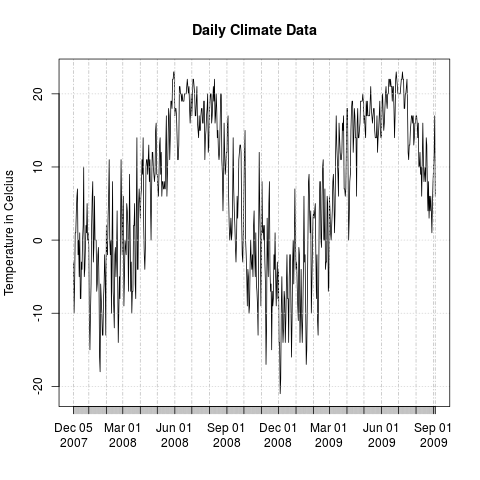
\includegraphics[width=.8\linewidth]{paper_figures/plot_m4_train.png}
\centering
\caption{The training data from the M4 forecasting competition}
\label{fig:m4_train}
\end{figure}
\doublespacing

This series has a distinct seasonality feature, which will give the forecasting tools in \pkg{mlr} a challenge. Figure~\ref{fig:m4_train} is what most would imagine when they think of a time series. There is a clear seasonal time trend with individual points moving about the annual seasons. The data can be found in the package \pkg{M4comp}~\cite{m4comp} under \code{M4[8836]}.

\subsection{Multivariate Forecasting Data}
This paper uses the EUStockMarkets data set from the \pkg{datasets}~\cite{datasets} package to showcase the multivariate forecasting tools. It contains a subset of daily DAX, SMI, CAC, and FTSE European stock indices from July 1st, 1991 to August 24th, 1998 totaling 1828 training observations and 32 test observations.

\singlespace
\begin{knitrout}
\definecolor{shadecolor}{rgb}{0.969, 0.969, 0.969}\color{fgcolor}\begin{kframe}
\begin{alltt}
\hlcom{# Read in Stock Market Data}
\hlkwd{data}\hlstd{(}\hlstr{"EuStockMarkets"}\hlstd{)}
\hlstd{EuStockMarkets.time} \hlkwb{=} \hlstd{lubridate}\hlopt{::}\hlkwd{date_decimal}\hlstd{(}
                \hlkwd{as.numeric}\hlstd{(}\hlkwd{time}\hlstd{(EuStockMarkets)))}
\hlstd{EuStockMarkets}  \hlkwb{=} \hlstd{xts}\hlopt{::}\hlkwd{xts}\hlstd{(}\hlkwd{as.data.frame}\hlstd{(EuStockMarkets),}
                           \hlkwc{order.by} \hlstd{= EuStockMarkets.time)}
\hlstd{eu.train} \hlkwb{=} \hlstd{EuStockMarkets[}\hlnum{1}\hlopt{:}\hlnum{1828}\hlstd{,]}
\hlstd{eu.test} \hlkwb{=} \hlstd{EuStockMarkets[}\hlnum{1829}\hlopt{:}\hlnum{1860}\hlstd{,]}
\end{alltt}
\end{kframe}
\end{knitrout}



\doublespacing

Figure~\ref{fig:eu_train} shows the plot of each series. Note that each stock index tends to follow a similar, but diverging, trend. This will be important to note when performing windowed cross-validation as it will be a real test to see how well the models adapt to what appears to be nonstationary data.

\begin{figure}[h!]
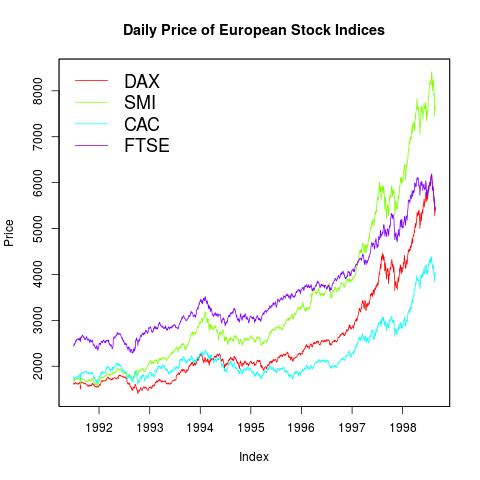
\includegraphics[width=\linewidth]{paper_figures/plot_eu_train.png}
\centering
\caption{The training data from the EuStockMarkets dataset}
\label{fig:eu_train}
\end{figure}

\section{Univariate and Multivariate Forecasting Tasks}
\label{sec:task}

\subsection{Univariate Tasks}
\label{sec:univarTask}
\pkg{mlr} uses the S3 object system to clearly define a predictive modeling task. Tasks contain the data and other relevant meta-information such as the task id and for supervised learning problems the target variable. Forecasting tasks are handled in \pkg{mlr} by the function \code{makeForecastRegrTask()}. The forecasting task inherets most of it's arguments from \code{makeRegrTask}, but has two additional arguments.

\begin{itemize}
\item[data:] Instead of a data frame, an xts object from \pkg{xts}~\cite{xts} containing the time series.
\item[frequency:] An integer representing the periodicity of the time series. For example, daily data with a weekly periodicity has a frequency of 7, daily data with a yearly periodicity has a frequency of 365, and weekly data with a yearly frequency has a periodicity of 52.
\end{itemize}

\singlespacing
\begin{knitrout}
\definecolor{shadecolor}{rgb}{0.969, 0.969, 0.969}\color{fgcolor}\begin{kframe}
\begin{alltt}
\hlkwd{library}\hlstd{(mlr)}
\hlstd{climate.task} \hlkwb{=} \hlkwd{makeForecastRegrTask}\hlstd{(}\hlkwc{id} \hlstd{=} \hlstr{"M4 Climate Data"}\hlstd{,}
                                 \hlkwc{data} \hlstd{= m4.train,}
                                 \hlkwc{target} \hlstd{=} \hlstr{"target_var"}\hlstd{,}
                                 \hlkwc{frequency} \hlstd{=} \hlnum{7L}\hlstd{)}
\hlstd{climate.task}
\end{alltt}
\begin{verbatim}
## Task: M4 Climate Data
## Type: fcregr
## Target: target_var
## Observations: 640
## Dates:
##  Start: 2007-12-05 
##  End:   2009-09-04
## Frequency: 7
## Features:
## numerics  factors  ordered 
##        0        0        0 
## Missings: FALSE
## Has weights: FALSE
## Has blocking: FALSE
\end{verbatim}
\end{kframe}
\end{knitrout}
\doublespacing
Like a regression task, this records the type of the learning problem and basic information about the data set such as the start and end dates, frequency, and whether there are missing values. Note that there are zero features in the task because there is only a target variable, which the model itself will use to build features.

\subsection{Multivariate Tasks}
\label{sec:multivarTask}

One common problem with forecasting is that it is hard to use additional explanatory variables or forecast multiple targets that are dependent on one another. If a model with exogenous variables is at time $t$ and is designed to predict ten periods in the future, it needs to know the values of the exogenous variables at time $t+10$, which is often not possible. A new set of models~\cite{BigVAR} which treats exogenous variables endogenously allows forecasters to not only forecast the target, but additional explanatory variables. Forecasting exogenous variables works by treating all the variables as targets, making them endogenous to the model. A multivariate forecasting task is created to hold the data and meta-information for the model. The function \code{makeMultiForecastRegrTask()} has the same arguments as \code{makeForecastRegrTask()} with one exception. The \code{target} argument can contain either a single target variable, multiple target variables, or \code{All} which treats all variables endogenously.

\singlespacing
\begin{knitrout}
\definecolor{shadecolor}{rgb}{0.969, 0.969, 0.969}\color{fgcolor}\begin{kframe}
\begin{alltt}
\hlstd{mfcregr.univar.task} \hlkwb{=} \hlkwd{makeMultiForecastRegrTask}\hlstd{(}\hlkwc{id} \hlstd{=} \hlstr{"bigvar"}\hlstd{,}
                                         \hlkwc{data} \hlstd{= eu.train,}
                                         \hlkwc{target} \hlstd{=} \hlstr{"FTSE"}\hlstd{,}
                                         \hlkwc{frequency} \hlstd{=} \hlnum{5L}\hlstd{)}
\hlstd{mfcregr.univar.task}
\end{alltt}
\begin{verbatim}
## Task: bigvar
## Type: mfcregr
## Target: FTSE
## Observations: 1828
## Dates:
##  Start: 1991-07-01 02:18:27 
##  End:   1998-07-10 22:09:13
## Frequency: 5
## Features:
## numerics  factors  ordered 
##        3        0        0 
## Missings: FALSE
## Has weights: FALSE
## Has blocking: FALSE
\end{verbatim}
\end{kframe}
\end{knitrout}
\doublespacing

Like \code{makeForecastRegrTask()}, \code{mfcregr.univar.task} has the standard output, but notice now that there are three features. Alternatively, \code{mfcregr.all.task} contains multiple target values with no features. The difference between each of these multivariate tasks is that \code{mfcregr.univar.task} will act similar to \code{makeForecastRegrTask()}, giving a univariate forecast output and evaluating the forecasts with univariate measures. When the target is \code{All} or multiple variables the trained model will forecast and output all series and use a multivariate form of the univariate measures. Though the results appear different, both of these tasks will still forecast all of the underlying series, which allows the model take in exogenous variables and treat them endogenously for n-step ahead forecasts that use additional explanatory variables.

\singlespacing
\begin{knitrout}
\definecolor{shadecolor}{rgb}{0.969, 0.969, 0.969}\color{fgcolor}\begin{kframe}
\begin{alltt}
\hlstd{mfcregr.all.task} \hlkwb{=} \hlkwd{makeMultiForecastRegrTask}\hlstd{(}\hlkwc{id} \hlstd{=} \hlstr{"bigvar"}\hlstd{,}
                                      \hlkwc{data} \hlstd{= eu.train,}
                                      \hlkwc{target} \hlstd{=} \hlstr{"all"}\hlstd{,}
                                      \hlkwc{frequency} \hlstd{=} \hlnum{5L}\hlstd{)}
\hlstd{mfcregr.all.task}
\end{alltt}
\begin{verbatim}
## Task: bigvar
## Type: mfcregr
## Target: DAX SMI CAC FTSE
## Observations: 1828
## Dates:
##  Start: 1991-07-01 02:18:27 
##  End:   1998-07-10 22:09:13
## Frequency: 5
## Features:
## numerics  factors  ordered 
##        0        0        0 
## Missings: FALSE
## Has weights: FALSE
## Has blocking: FALSE
\end{verbatim}
\end{kframe}
\end{knitrout}
\doublespacing

\section{Building a forecast learner}
\label{seq:build}
\subsection{Univariate Forecasting}
\label{seq:buildAndTuneUni}

The \code{makeLearner()} function provides a structured model building framework to the several forecasting models currently implemented in \pkg{mlr}. This section will build an exponential smoothing state space model (ETS)~\cite{etsMod} to show how to create forecasting models in \pkg{mlr}.

ETS is one of the most popular forecasting models and is available in \pkg{mlr} along with models such as BATS, ARIMA, TBATS, several GARCH variants, and autoregressive neural networks. Section~\ref{sec:preprocAR} uses preprocessing features to develop arbitrary supervised machine learning models in the context of forecasting. An ETS model is created by calling the function \code{makeLearner()}, supplying the class of learner, the number of steps to forecast, and any additional arguments to be passed to \code{ets()} from \pkg{forecast}.

%\footnote{Possible arguments to the model can be found by using \code{getLearnerParamSet("fcregr.tbats")}.}
\singlespacing
\begin{knitrout}
\definecolor{shadecolor}{rgb}{0.969, 0.969, 0.969}\color{fgcolor}\begin{kframe}
\begin{alltt}
\hlstd{ets.mod} \hlkwb{=}\hlkwd{makeLearner}\hlstd{(}\hlkwc{cl} \hlstd{=} \hlstr{"fcregr.ets"}\hlstd{,} \hlkwc{model} \hlstd{=} \hlstr{"AZA"}\hlstd{,}
                     \hlkwc{h} \hlstd{=} \hlnum{35}\hlstd{,} \hlkwc{predict.type} \hlstd{=} \hlstr{"response"}\hlstd{)}
\hlstd{ets.mod}
\end{alltt}
\begin{verbatim}
## Learner fcregr.ets from package forecast
## Type: fcregr
## Name: Exponential smoothing state space model; Short name: ets
## Class: fcregr.ets
## Properties: numerics,quantile
## Predict-Type: response
## Hyperparameters: model=AZA,h=35
\end{verbatim}
\end{kframe}
\end{knitrout}
\doublespacing

The \code{predict.type} for forecasting models can either be a point estimate (\code{response}) or point estimates with quantiles of confidence intervals (\code{quantile}). The function \code{train()} is called, supplying both the learner and task to build the final model over the full data set.

\singlespace
\begin{knitrout}
\definecolor{shadecolor}{rgb}{0.969, 0.969, 0.969}\color{fgcolor}\begin{kframe}
\begin{alltt}
\hlstd{train.ets} \hlkwb{=} \hlkwd{train}\hlstd{(}\hlkwc{learner} \hlstd{= ets.mod,} \hlkwc{task} \hlstd{= climate.task )}
\hlstd{train.ets}
\end{alltt}
\begin{verbatim}
## Model for learner.id=fcregr.ets; learner.class=fcregr.ets
## Trained on: task.id = M4 Climate Data; obs = 640; features = 0
## Hyperparameters: model=AZA,h=35
\end{verbatim}
\end{kframe}
\end{knitrout}
\doublespace

The forecasts are generated by calling \code{predict()}. Optionally, supplying the test data as an additional argument will allow \pkg{mlr} to return an object containing meta information for the forecasts along with the prediction and test data in columns \code{truth} and \code{response}, respectively.

\singlespacing
\begin{knitrout}
\definecolor{shadecolor}{rgb}{0.969, 0.969, 0.969}\color{fgcolor}\begin{kframe}
\begin{alltt}
\hlstd{predict.ets} \hlkwb{=} \hlkwd{predict}\hlstd{(train.ets,} \hlkwc{newdata} \hlstd{= m4.test)}
\hlstd{predict.ets}
\end{alltt}
\begin{verbatim}
## Prediction: 35 observations
## predict.type: response
## threshold: 
## time: 0.00
##            truth response
## 2009-09-06     7 7.679805
## 2009-09-07    12 7.490629
## 2009-09-08    14 7.227584
## 2009-09-09    10 8.283864
## 2009-09-10    10 8.795217
## 2009-09-11    16 8.184962
## ... (35 rows, 2 cols)
\end{verbatim}
\end{kframe}
\end{knitrout}
\doublespacing

The model is evaluated by calling \code{performance()} with the Mean Absolute Scaled Error (MASE)~\cite{Hyndman2006} measure.

\singlespacing
\begin{knitrout}
\definecolor{shadecolor}{rgb}{0.969, 0.969, 0.969}\color{fgcolor}\begin{kframe}
\begin{alltt}
\hlkwd{performance}\hlstd{(predict.ets,} \hlkwc{measure} \hlstd{= mase,}
            \hlkwc{task} \hlstd{= climate.task)}
\end{alltt}
\begin{verbatim}
##      mase 
## 0.6718168
\end{verbatim}
\end{kframe}
\end{knitrout}
\doublespacing
MASE has favorable properties for calculating forecast errors relative to measures such as root mean squared error or median relative absolute error. Arguably one of the most important features, it is very interpretable. Let $y_t$ and $\tilde{y}_t$ be the target variable and prediction at time $t$ with $\epsilon_t = y_t - \tilde{y}_t$ being the forecast error. Then MASE is calculated as

\begin{equation}
\text{MASE} = \frac{\sum_{t=1}^T |\epsilon_t|}{\frac{T}{T-1} \sum_{t=2}^T |y_{t, \text{insample}} - y_{t-1, \text{insample}}|}
\end{equation}

Where the denominator is the one step ahead naive forecast from the training data. When the numerator is equal to the denominator, the model performs as well as a simple naive forecast method. A MASE score greater than one indicates the model is performing worse than the naive forecasting method while scores less than one mean the model is performing better than the naive forecasting method.

The scale invariance of MASE means that it is independent of the scale of the data and allows model comparison across data sets. The scale invariance of MASE has made it a favorite for comparing the accuracy of forecast methods~\cite{noteMase} across datasets. While scaling in measures such as the Mean Absolute Percentage Error can cause poor behavior as the target variable goes to zero, MASE does not become skewed when the target variable approaches zero. Having good properties near zero allows the use of MASE in situations in which zeros occur frequently or zero is not meaningful such as predicting temperature. The model does a successful job of catching the downward trend, but figure~\ref{fig:ets_train} shows the downward bias of the model which does not allow it to account for the sharp upward swings.

\singlespacing


\doublespacing

\begin{figure}[h!]
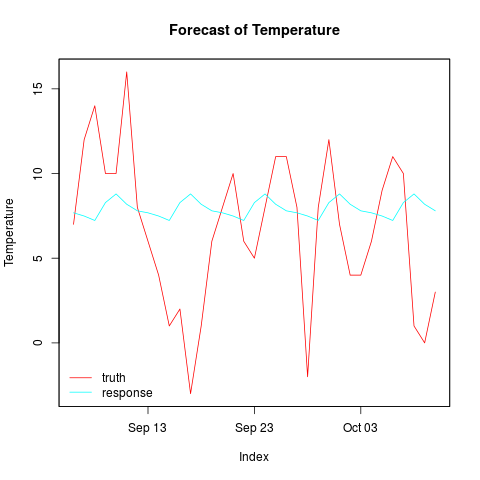
\includegraphics[width=\linewidth]{paper_figures/plot_ets_train.png}
\centering
\caption{The forecasts response from ets against the testing weather data}
\label{fig:ets_train}
\end{figure}

\subsection{Updating Forecast Models}

 Forecasting models are designed to predict the next $n$ values that will appear in the series. Without a way to update the model with new data, the model will have to be completely rebuilt for each new set of forecasts. The \code{updateModel} function allows forecasters to avoid the expensive cost of retraining the entire forecasting model. The function updates the model with new points which then allows for updated forecasts.

\singlespacing
\begin{knitrout}
\definecolor{shadecolor}{rgb}{0.969, 0.969, 0.969}\color{fgcolor}\begin{kframe}
\begin{alltt}
\hlstd{update.ets} \hlkwb{=} \hlkwd{updateModel}\hlstd{(train.ets, climate.task,}
                           \hlkwc{newdata} \hlstd{= m4.test)}
\hlkwd{predict}\hlstd{(update.ets,} \hlkwc{task} \hlstd{= climate.task)}
\end{alltt}
\begin{verbatim}
## Prediction: 35 observations
## predict.type: response
## threshold: 
## time: 0.00
##                      response
## 2009-09-04 23:59:54 2.0716814
## 2009-09-05 23:59:48 1.8703286
## 2009-09-06 23:59:43 3.4973941
## 2009-09-07 23:59:37 3.4825407
## 2009-09-08 23:59:31 0.4462708
## 2009-09-09 23:59:26 2.3802832
## ... (35 rows, 1 cols)
\end{verbatim}
\end{kframe}
\end{knitrout}
\doublespacing

All univariate forecasting models have access to the \code{updateModel()} function. Future versions of \code{mlr} will also include online machine learning models that can be updated as new data comes in.

\subsection{Multivariate Forecasting}
\label{seq:buildAndTuneMulti}

Multivariate forecasting in \pkg{mlr} uses the package \pkg{BigVAR}~\cite{bigvarpaper}. \pkg{BigVAR} allows for estimation of high dimensional time series through methods such as structured Lasso penalties to find the optimal autoregressive structures through cross-sections and time.

\singlespacing
\begin{knitrout}
\definecolor{shadecolor}{rgb}{0.969, 0.969, 0.969}\color{fgcolor}\begin{kframe}
\begin{alltt}
\hlstd{bigvar.mod} \hlkwb{=} \hlkwd{makeLearner}\hlstd{(}\hlstr{"mfcregr.BigVAR"}\hlstd{,}\hlkwc{p} \hlstd{=} \hlnum{25}\hlstd{,}
                         \hlkwc{struct} \hlstd{=} \hlstr{"SparseLag"}\hlstd{,}
                         \hlkwc{gran} \hlstd{=} \hlkwd{c}\hlstd{(}\hlnum{50}\hlstd{,} \hlnum{60}\hlstd{),}\hlkwc{h} \hlstd{=} \hlnum{35}\hlstd{,} \hlkwc{n.ahead} \hlstd{=} \hlnum{35}\hlstd{)}
\end{alltt}
\end{kframe}
\end{knitrout}
\doublespacing

This section uses the multivariate forecast task which has all variables as targets, while section~\ref{sub:multiStack} performs the single target multivariate forecast with a stacked predictor. Multiforecast regressions operate the same as other supervised models, supplying a task and learner to \code{train()}.

\singlespacing
\begin{knitrout}
\definecolor{shadecolor}{rgb}{0.969, 0.969, 0.969}\color{fgcolor}\begin{kframe}
\begin{alltt}
\hlstd{train.bigvar} \hlkwb{=} \hlkwd{train}\hlstd{(}\hlkwc{learner} \hlstd{= bigvar.mod,}
                     \hlkwc{task} \hlstd{= mfcregr.all.task )}
\hlstd{train.bigvar}
\end{alltt}
\end{kframe}
\end{knitrout}

\begin{knitrout}
\definecolor{shadecolor}{rgb}{0.969, 0.969, 0.969}\color{fgcolor}\begin{kframe}
\begin{verbatim}
## Model for learner.id=mfcregr.BigVAR; learner.class=mfcregr.BigVAR
## Trained on: task.id = bigvar; obs = 1828; features = 0
## Hyperparameters: p=25,struct=SparseLag,gran=50,60,h=35,n.ahead=35
\end{verbatim}
\end{kframe}
\end{knitrout}
\doublespacing

Predictions for \code{multiForecast} methods have a similar output to \code{multiclass} methods, returning multiple truth and response variables. For multivariate forecasts, a multivariate version of MASE takes the mean of each MASE score for the individual variables as the performance measure.

\begin{equation}
\text{MultiMASE} = \frac{\sum_{i=1}^m \text{MASE}_i}{m}
\end{equation}

given that $m$ is the number of variables that are forecast.

\singlespacing
\begin{knitrout}
\definecolor{shadecolor}{rgb}{0.969, 0.969, 0.969}\color{fgcolor}\begin{kframe}
\begin{alltt}
\hlstd{predict.bigvar} \hlkwb{=} \hlkwd{predict}\hlstd{(train.bigvar,} \hlkwc{newdata} \hlstd{= eu.test)}
\hlstd{predict.bigvar}
\end{alltt}
\begin{verbatim}
## Prediction: 32 observations
## predict.type: response
## threshold: 
## time: 0.02
##                     truth.DAX truth.SMI truth.CAC truth.FTSE response.DAX
## 1998-07-12 07:50:46   5905.15    8047.3    4252.1     5960.2     5852.841
## 1998-07-13 17:32:18   5961.45    8099.0    4304.4     5988.4     5820.194
## 1998-07-15 03:13:50   5942.06    8166.0    4311.1     5990.3     5801.712
## 1998-07-16 12:55:23   5975.88    8160.0    4333.1     6003.4     5790.565
## 1998-07-17 22:36:55   6018.89    8227.2    4339.9     6009.6     5781.540
## 1998-07-19 08:18:27   6000.84    8205.0    4319.2     5969.7     5772.087
##                     response.SMI response.CAC response.FTSE
## 1998-07-12 07:50:46     7982.503     4192.149      5997.825
## 1998-07-13 17:32:18     7960.779     4153.550      6037.958
## 1998-07-15 03:13:50     7955.264     4130.674      6063.687
## 1998-07-16 12:55:23     7958.119     4115.612      6083.094
## 1998-07-17 22:36:55     7965.061     4103.302      6100.075
## 1998-07-19 08:18:27     7973.586     4091.154      6116.419
## ... (32 rows, 8 cols)
\end{verbatim}
\begin{alltt}
\hlkwd{performance}\hlstd{(predict.bigvar, multivar.mase,}
            \hlkwc{task} \hlstd{= mfcregr.all.task)}
\end{alltt}
\begin{verbatim}
## multivar.mase 
##       12.7678
\end{verbatim}
\end{kframe}
\end{knitrout}


\begin{figure}[H]
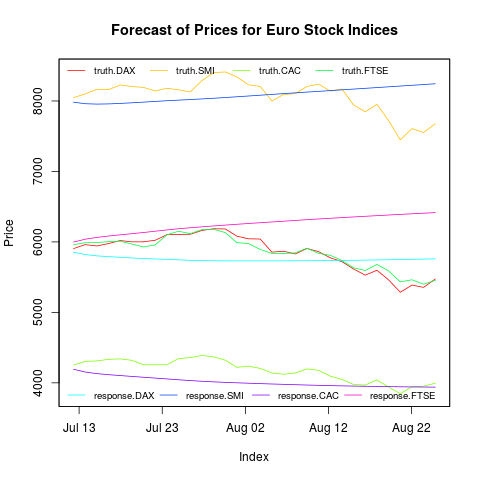
\includegraphics[width=.8\linewidth]{paper_figures/plot_bigvar_train.png}
\centering
\caption{The forecasts response from BigVAR against the true test stock index data}
\label{fig:bigvar_train}
\end{figure}
\doublespacing

\section{Resampling with Time}
\label{sec:resamp}


While ETS is one of the most popular time series models the error type, trend type, season type, and whether to include a damped or multiplicative trend can be a subjective process that will almost always lead to a sub-optimal model selection. One of the first proposals for automated forecasting methods comes from~\cite{hannanOrder} for automatic order selection of ARIMA models. Innovations are obtained by fitting high order autoregressive models to the data and then computing the likelihood of potential models through a series of standard regression. Proprietary algorithms from software such as \proglang{Forecast Pro}~\cite{forecastpro} and \proglang{Autobox}~\cite{reillyautobox} are well known and have performed to high standards in competitions such as the M3 forecasting competition~\cite{Makridakis2000451}. One of the most prominent R packages for automated forecasting is \pkg{forecast}~\cite{HyndForecast} which contains several methods for automated forecasting including exponential smoothing based methods and step-wise algorithms for finding optimal ARIMA models.

Forecasting in \pkg{mlr} takes a machine learning approach, creating a parameter set for a given model and using an optimization method to search over the parameter space. The forecasting extension of \pkg{mlr} includes growing and fixed window resampling schemes to train over the possible models. Resampling schemes such as cross-validation and bootstrapping are common in machine learning for dealing with the bias-variance tradeoff~\cite{Friedman1997}~\cite{rodriguezkfold}. When there is a time component to the data, windowing schemes are useful in allowing a valid resampling scheme while still accounting for the time properties of the series. Figure~\ref{fig:caret} gives an example of fixed and growing window cross validation. Let $h$ be a forecast horizon where the index of the starting and end points of the training data are $\text{start}_i$ and $\text{end}_i$ where $i$ is the index for each window. The first model will train on data between $\text{start}_i$ and $\text{end}_i$ while testing on data indexed between $\text{end}_i + h$. After each iteration the window slides forward $h$ steps such that $\text{end}_{i+1} = \text{end}_{i} + h$. In the case of the fixed window, the starting index will also shift such that $\text{start}_{i+1} = \text{start}_{i} + h$ while $\text{start}_i$ will remain constant in the growing window case. This type of growing and fixed window resampling~\cite{hyndman2014forecasting} is now available in the \code{resampling()} function of \pkg{mlr}.

\begin{figure}[h!]
  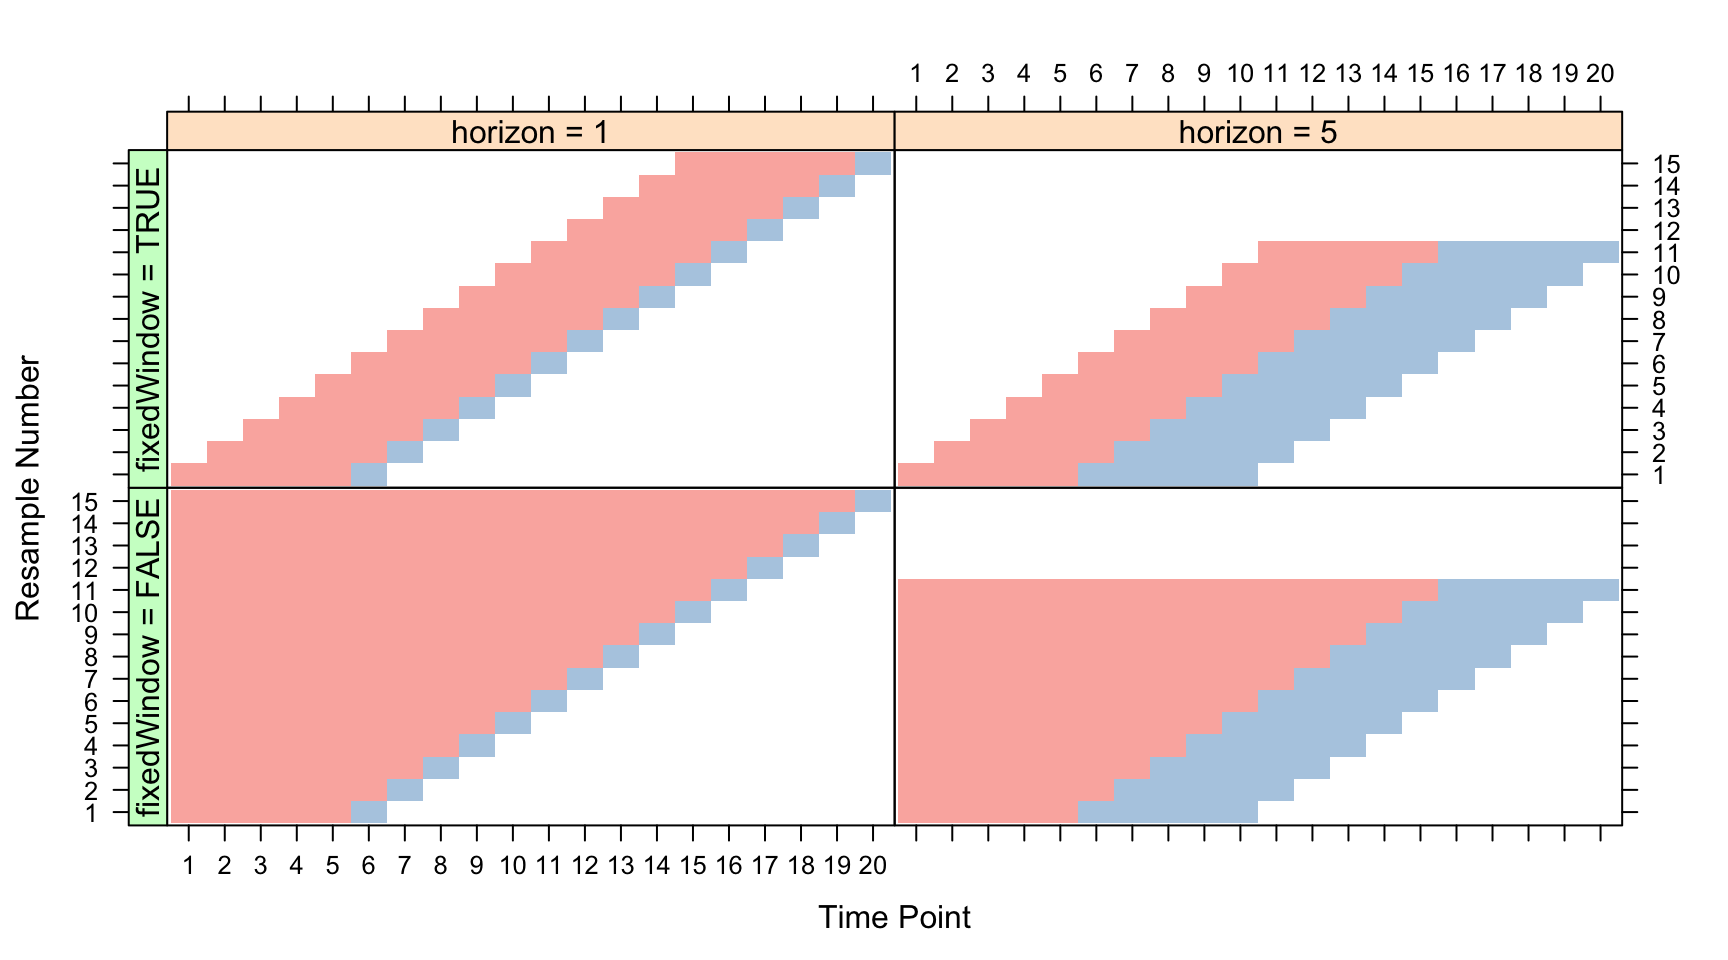
\includegraphics[width=\linewidth]{paper_figures/windowing_pic_caret}
  \centering
  \caption{Resampling with a window scheme as exampled by \pkg{caret}~\cite{windowingcaret}. The top graphs are fixed window cross validation while the bottom graphs are growing window cross validation. }
  \label{fig:caret}
\end{figure}

To create a windowing resampling process, the function \code{makeResampleDesc()} uses the resampling type, the horizon, initial window, the length of the series, and an optional argument to skip over some windows for the sake of time.

\singlespacing
\begin{knitrout}
\definecolor{shadecolor}{rgb}{0.969, 0.969, 0.969}\color{fgcolor}\begin{kframe}
\begin{alltt}
\hlstd{resampDesc} \hlkwb{=} \hlkwd{makeResampleDesc}\hlstd{(}\hlstr{"GrowingCV"}\hlstd{,} \hlkwc{horizon} \hlstd{=} \hlnum{35L}\hlstd{,}
                          \hlkwc{initial.window} \hlstd{=} \hlnum{.6}\hlstd{,}
                          \hlkwc{size} \hlstd{=} \hlkwd{nrow}\hlstd{(}\hlkwd{getTaskData}\hlstd{(climate.task)),}
                          \hlkwc{skip} \hlstd{=} \hlnum{.038}\hlstd{)}
\hlstd{resampDesc}
\end{alltt}
\begin{verbatim}
## Window description:
##  growing with 10 iterations:
##  384 observations in initial window and 35 horizon.
## Predict: test
## Stratification: FALSE
\end{verbatim}
\end{kframe}
\end{knitrout}
\doublespacing

The methods in package \pkg{ParamHelpers}~\cite{paramhelper} allow \pkg{mlr} to have a simple and rigorous interface for creating parameter spaces. There are several types of tools to help search the parameter space including grid search, random search~\cite{Bergstra}, iterated F-racing~\cite{irace}, Simulated Annealing, and CMA-ES~\cite{cmaes}  to search the parameter space for the most optimal model. This ETS model uses only discrete and logical parameters, however functions are available for numeric, integer, numeric vectors, and several other types of parameters.


\singlespacing
\begin{knitrout}
\definecolor{shadecolor}{rgb}{0.969, 0.969, 0.969}\color{fgcolor}\begin{kframe}
\begin{alltt}
\hlstd{parSet} \hlkwb{=} \hlkwd{makeParamSet}\hlstd{(}
  \hlkwd{makeDiscreteParam}\hlstd{(}\hlstr{"model"}\hlstd{,} \hlkwc{values} \hlstd{=} \hlkwd{c}\hlstd{(}\hlstr{"ANN"}\hlstd{,} \hlstr{"MNN"}\hlstd{,} \hlstr{"ZNN"}\hlstd{,}
                                        \hlstr{"AAN"}\hlstd{,} \hlstr{"MAN"}\hlstd{,} \hlstr{"ZAN"}\hlstd{,}
                                        \hlstr{"AMN"}\hlstd{,} \hlstr{"MMN"}\hlstd{,} \hlstr{"ZMN"}\hlstd{,}
                                        \hlstr{"AZN"}\hlstd{,} \hlstr{"MZN"}\hlstd{,} \hlstr{"ZZN"}\hlstd{,}
                                        \hlstr{"ANA"}\hlstd{,} \hlstr{"MNA"}\hlstd{,} \hlstr{"ZNA"}\hlstd{,}
                                        \hlstr{"AAA"}\hlstd{,} \hlstr{"MAA"}\hlstd{,} \hlstr{"ZAA"}\hlstd{,}
                                        \hlstr{"AMA"}\hlstd{,} \hlstr{"MMA"}\hlstd{,} \hlstr{"ZMA"}\hlstd{,}
                                        \hlstr{"AZA"}\hlstd{)),}
  \hlkwd{makeLogicalParam}\hlstd{(}\hlstr{"damped"}\hlstd{),}
  \hlkwd{makeLogicalParam}\hlstd{(}\hlstr{"additive.only"}\hlstd{),}
  \hlkwd{makeLogicalParam}\hlstd{(}\hlstr{"biasadj"}\hlstd{),}
  \hlkwd{makeDiscreteParam}\hlstd{(}\hlstr{"opt.crit"}\hlstd{,} \hlkwc{values} \hlstd{=} \hlkwd{c}\hlstd{(}\hlstr{"mase"}\hlstd{,} \hlstr{"amse"}\hlstd{,}
                                           \hlstr{"sigma"}\hlstd{,} \hlstr{"mae"}\hlstd{,}
                                           \hlstr{"lik"}\hlstd{)),}
  \hlkwd{makeDiscreteParam}\hlstd{(}\hlstr{"ic"}\hlstd{,} \hlkwc{values} \hlstd{=} \hlkwd{c}\hlstd{(}\hlstr{"aicc"}\hlstd{,} \hlstr{"aic"}\hlstd{,} \hlstr{"bic"}\hlstd{)),}
  \hlkwd{makeLogicalParam}\hlstd{(}\hlstr{"allow.multiplicative.trend"}\hlstd{)}
\hlstd{)}

\hlcom{#Specify tune by grid estimation}
\hlstd{ctrl} \hlkwb{=} \hlkwd{makeTuneControlIrace}\hlstd{(}\hlkwc{maxExperiments} \hlstd{=} \hlnum{500L}\hlstd{)}
\end{alltt}
\end{kframe}
\end{knitrout}
\doublespacing

Using \code{tuneParams()}, the model is tuned for the task using the specified resampling scheme, parameter set, tune control, and measure. This tuning task uses MASE~\cite{Hyndman2006} as a measure of performance \footnote{If a frequency is defined in the task, the seasonal MASE score will be used.}. The model is also tuned in parallel using the package \pkg{parallelMap}~\cite{parallel} for it's built in compatibility with \pkg{mlr}.

\singlespacing
\begin{knitrout}
\definecolor{shadecolor}{rgb}{0.969, 0.969, 0.969}\color{fgcolor}\begin{kframe}
\begin{alltt}
\hlcom{#Tune the ETS Model}
\hlkwd{library}\hlstd{(}\hlstr{"parallelMap"}\hlstd{)}
\hlkwd{parallelStart}\hlstd{(}\hlstr{"multicore"}\hlstd{,} \hlnum{8}\hlstd{)}
\hlkwd{configureMlr}\hlstd{(}\hlkwc{on.learner.error} \hlstd{=} \hlstr{"warn"}\hlstd{)}
\hlkwd{set.seed}\hlstd{(}\hlnum{1234}\hlstd{)}
\hlstd{etsTune} \hlkwb{=} \hlkwd{tuneParams}\hlstd{(}\hlkwd{makeLearner}\hlstd{(}\hlstr{"fcregr.ets"}\hlstd{,} \hlkwc{h} \hlstd{=} \hlnum{35}\hlstd{),}
                       \hlkwc{task} \hlstd{= climate.task,}
                       \hlkwc{resampling} \hlstd{= resampDesc,} \hlkwc{par.set} \hlstd{= parSet,}
                       \hlkwc{control} \hlstd{= ctrl,} \hlkwc{measures} \hlstd{= mase)}
\hlkwd{parallelStop}\hlstd{()}
\hlcom{# Output the test mean of best model}
\hlstd{etsTune}\hlopt{$}\hlstd{y}
\end{alltt}
\end{kframe}
\end{knitrout}



\begin{knitrout}
\definecolor{shadecolor}{rgb}{0.969, 0.969, 0.969}\color{fgcolor}\begin{kframe}
\begin{verbatim}
## mase.test.mean 
##      0.8064303
\end{verbatim}
\end{kframe}
\end{knitrout}

\doublespace

Using \pkg{mlr}'s built in plotting routines the tuning parameters can be analyzed\footnote{Because of constraints which do not allow logical types in the partial dependence plots, the below code takes all of the logical parameters from \code{etsTune} and coerces them to be numeric} graphically using partial dependence plots~\cite{partialdep}.

\singlespace

\begin{knitrout}
\definecolor{shadecolor}{rgb}{0.969, 0.969, 0.969}\color{fgcolor}\begin{kframe}
\begin{alltt}
\hlcom{# Make data for dependence plot}
\hlstd{ets.hyp} \hlkwb{=} \hlkwd{generateHyperParsEffectData}\hlstd{(etsTune,} \hlkwc{partial.dep} \hlstd{=} \hlnum{TRUE}\hlstd{,}
                                        \hlkwc{trafo} \hlstd{=} \hlnum{TRUE}\hlstd{)}
\end{alltt}
\end{kframe}
\end{knitrout}



\begin{knitrout}
\definecolor{shadecolor}{rgb}{0.969, 0.969, 0.969}\color{fgcolor}\begin{kframe}
\begin{alltt}
\hlcom{# Making graphics}
\hlkwd{plotHyperParsEffect}\hlstd{(ets.hyp,} \hlkwc{x}\hlstd{=} \hlstr{"model"}\hlstd{,} \hlkwc{y} \hlstd{=} \hlstr{"mase.test.mean"}\hlstd{,}
                     \hlkwc{plot.type} \hlstd{=} \hlstr{"line"}\hlstd{,}
                     \hlkwc{partial.dep.learn} \hlstd{=} \hlstr{"regr.randomForest"}\hlstd{)} \hlopt{+}
  \hlkwd{theme_tufte}\hlstd{()}\hlopt{+} \hlkwd{theme}\hlstd{(}\hlkwc{text} \hlstd{=} \hlkwd{element_text}\hlstd{(}\hlkwc{size}\hlstd{=}\hlnum{20}\hlstd{))}
\hlkwd{plotHyperParsEffect}\hlstd{(ets.hyp,} \hlkwc{x}\hlstd{=} \hlstr{"opt.crit"}\hlstd{,} \hlkwc{y} \hlstd{=} \hlstr{"mase.test.mean"}\hlstd{,}
                     \hlkwc{plot.type} \hlstd{=} \hlstr{""}\hlstd{,}
                     \hlkwc{partial.dep.learn} \hlstd{=} \hlstr{"regr.randomForest"}\hlstd{)} \hlopt{+}
  \hlkwd{theme_tufte}\hlstd{()}\hlopt{+} \hlkwd{theme}\hlstd{(}\hlkwc{text} \hlstd{=} \hlkwd{element_text}\hlstd{(}\hlkwc{size}\hlstd{=}\hlnum{20}\hlstd{))}
\end{alltt}
\end{kframe}
\end{knitrout}



\begin{figure}[h!]
\centering
\begin{minipage}{.5\textwidth}
  \centering
  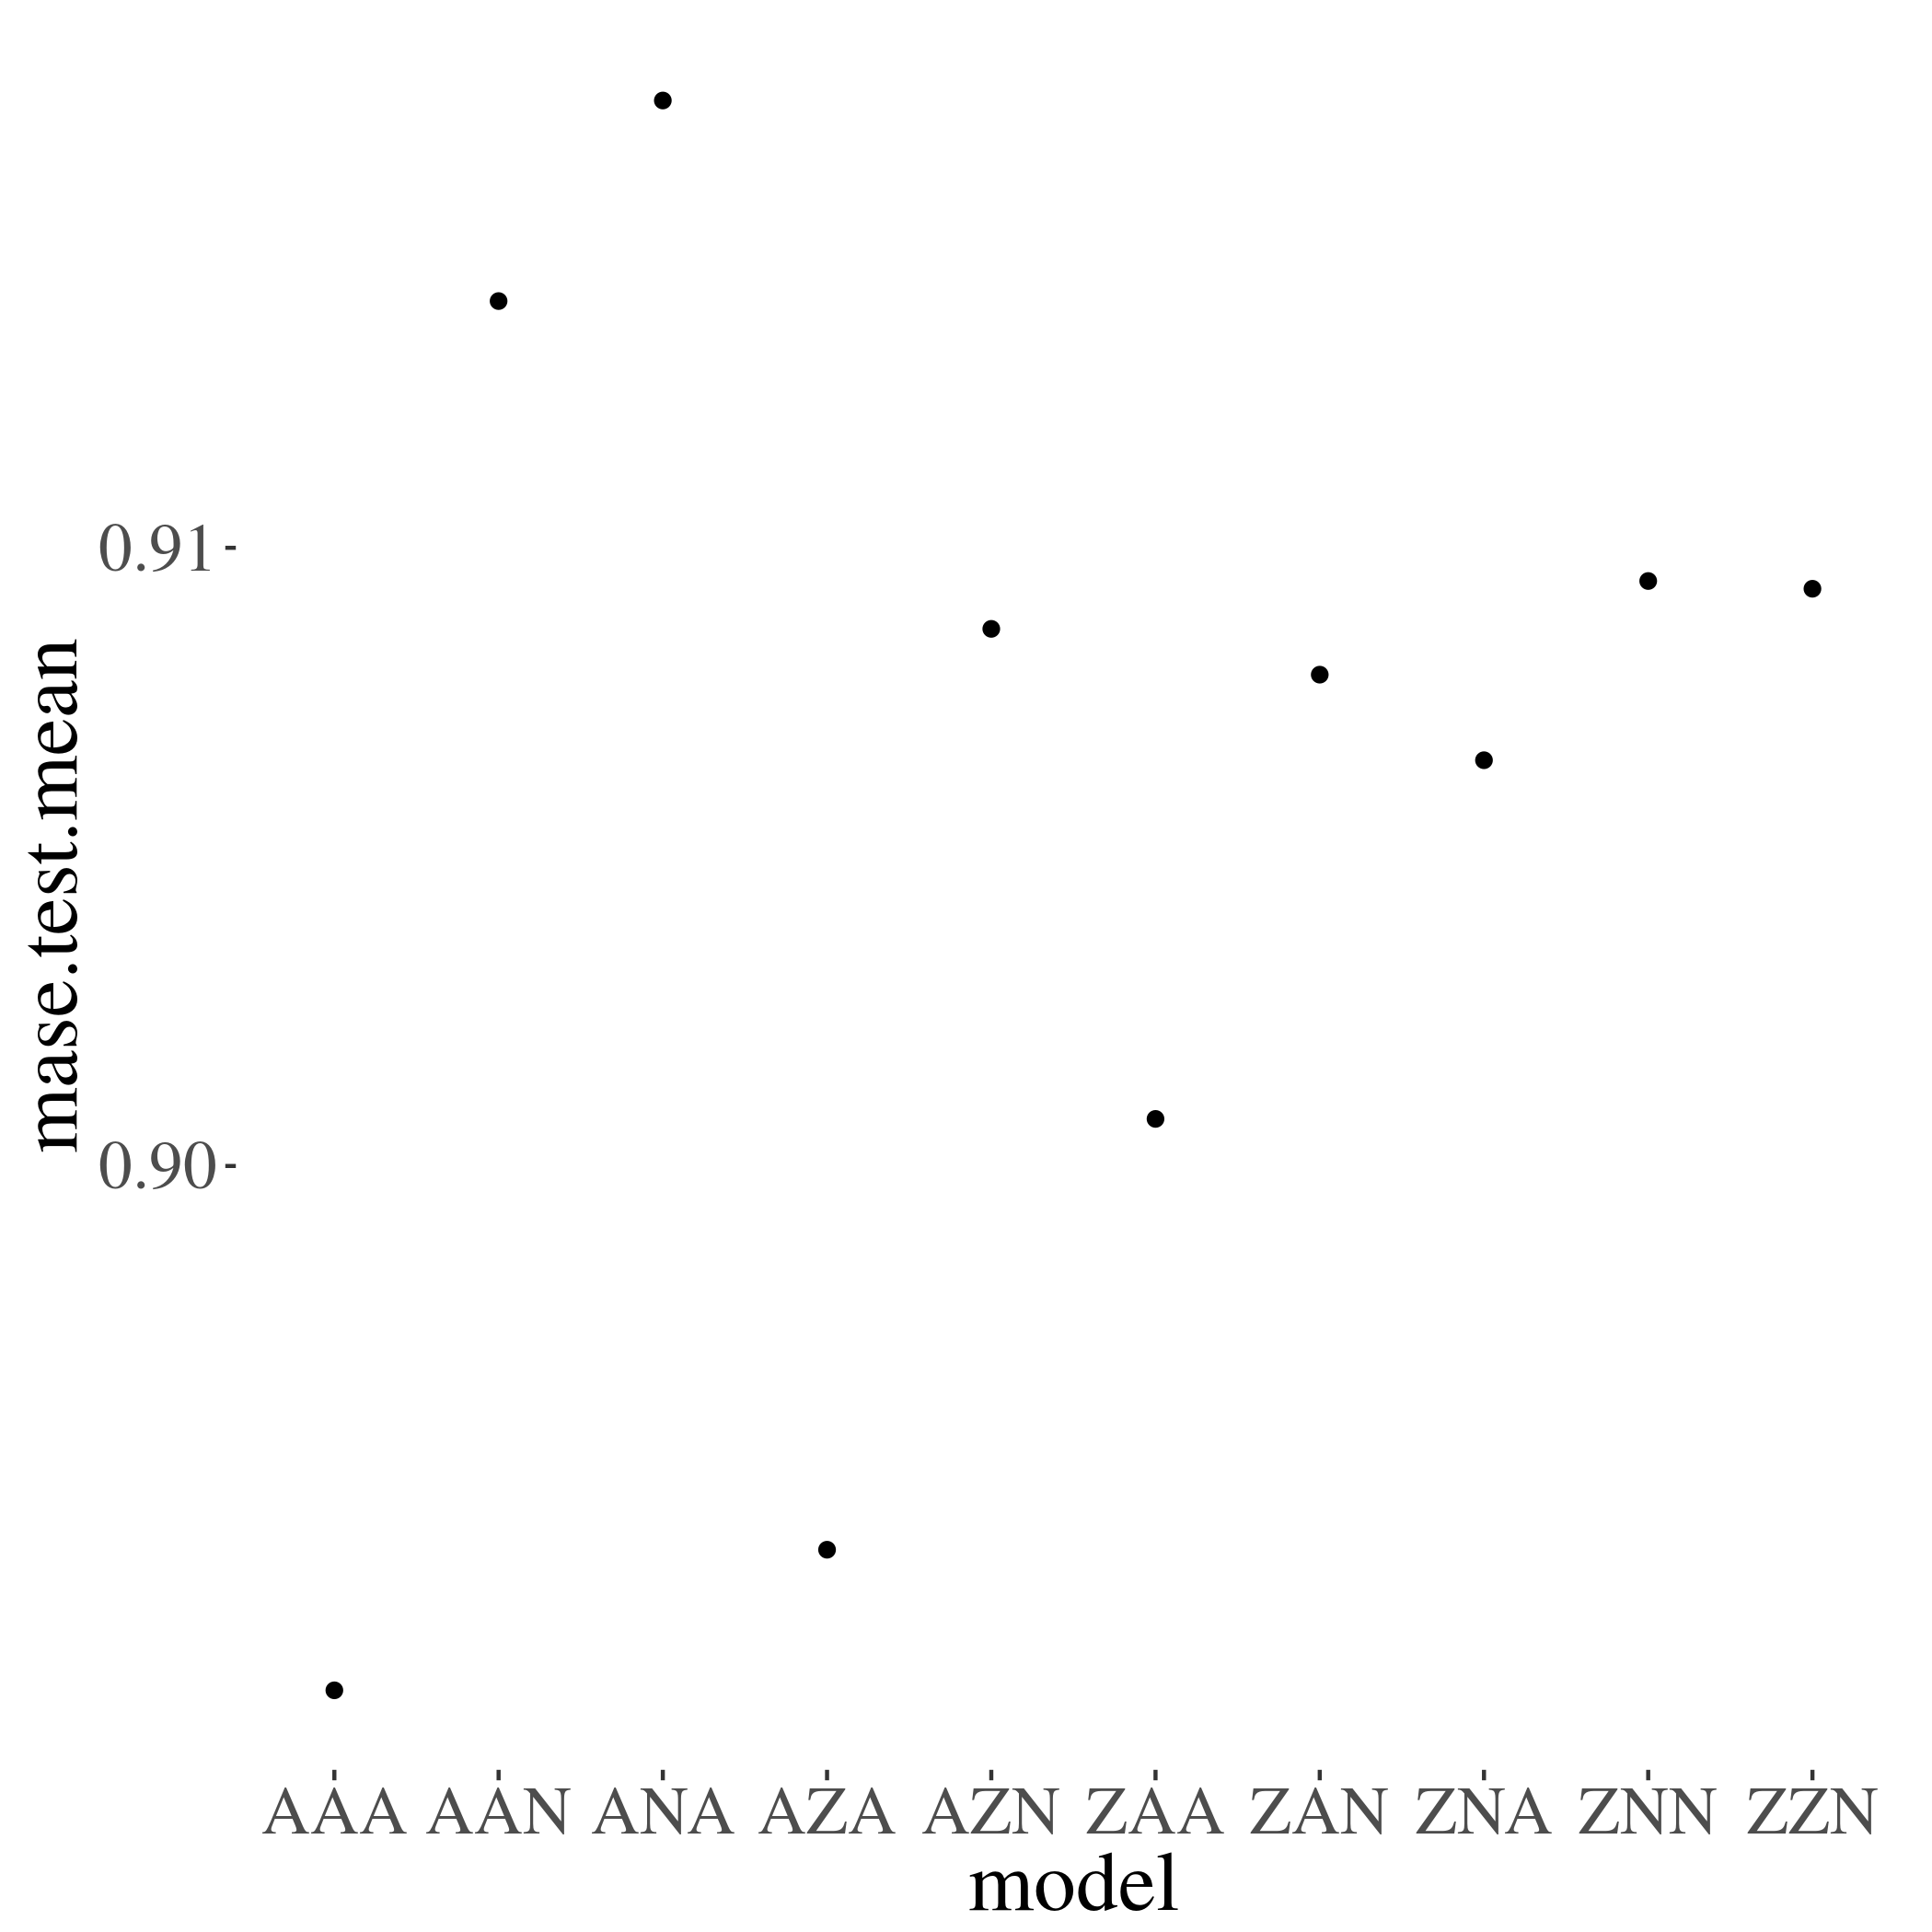
\includegraphics[width=\linewidth]{paper_figures/ets_dep_plot_max_q.png}
  \label{fig:etsDep1}
\end{minipage}%
\begin{minipage}{.5\textwidth}
  \centering
  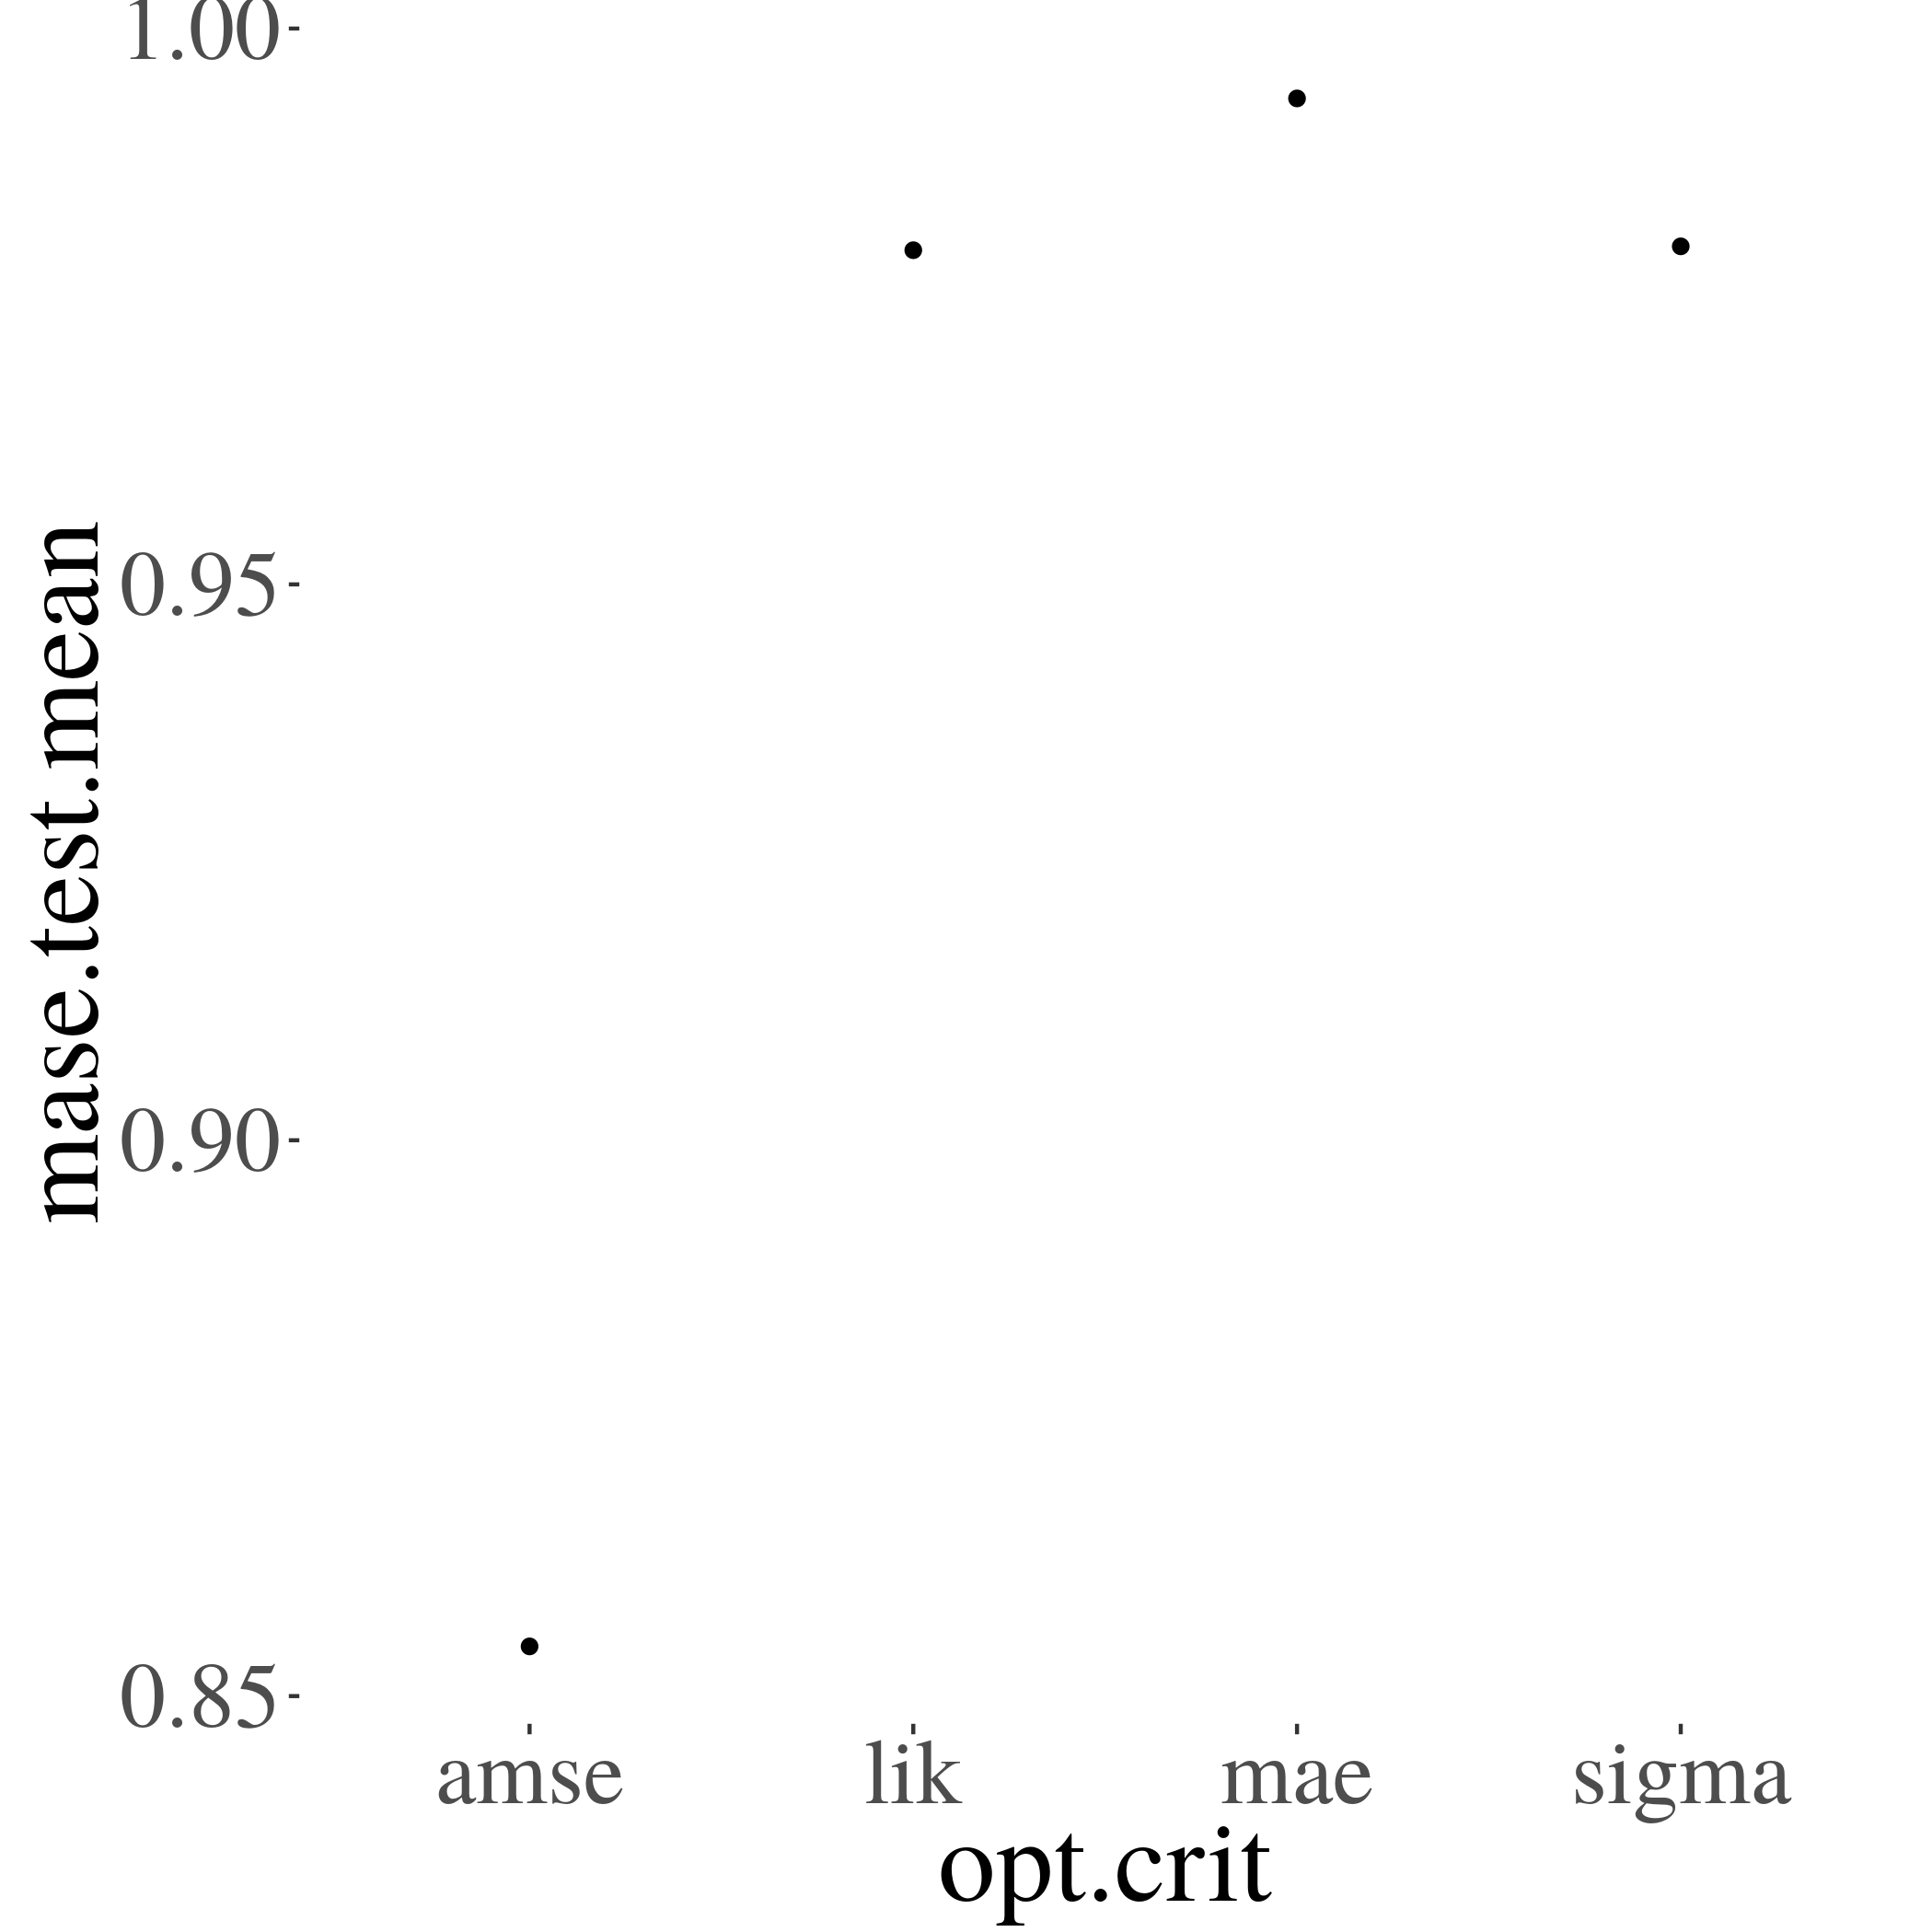
\includegraphics[width=\linewidth]{paper_figures/ets_dep_plot_max_p.png}
  \label{fig:etsDep2}
\end{minipage}
\caption{The figure on the left shows the dependence of the MASE score averaged over all windows for each value of ets models. The figure on the right does the same, but for the optimization criteria.}
\end{figure}

\doublespacing

Note that in figure 6 the best score in terms of model, independent of everything else, is AAA. This differs from the optimal model passed from \code{tuneParams()} because the interactions of the AZA model with the other hyperparameters produces a better model. The best model's parameters are extracted using \code{setHyperPars()} and passed to \code{train()} to go over the full data set.

\singlespacing
\begin{knitrout}
\definecolor{shadecolor}{rgb}{0.969, 0.969, 0.969}\color{fgcolor}\begin{kframe}
\begin{alltt}
\hlcom{# Train best model over full data}
\hlstd{ets.lrn} \hlkwb{=} \hlkwd{setHyperPars}\hlstd{(}\hlkwd{makeLearner}\hlstd{(}\hlstr{"fcregr.ets"}\hlstd{,}
                                     \hlkwc{h} \hlstd{=} \hlnum{35}\hlstd{),}
                         \hlkwc{par.vals} \hlstd{= etsTune}\hlopt{$}\hlstd{x)}
\hlstd{ets.final} \hlkwb{=} \hlkwd{train}\hlstd{(ets.lrn, climate.task)}
\end{alltt}
\end{kframe}
\end{knitrout}
\doublespacing

A prediction object is created by passing the model and optional testing data to \code{predict()} while the performance of the model can be evaluated by calling \code{performance()}.

\singlespacing
\begin{knitrout}
\definecolor{shadecolor}{rgb}{0.969, 0.969, 0.969}\color{fgcolor}\begin{kframe}
\begin{alltt}
\hlstd{climate.pred} \hlkwb{=} \hlkwd{predict}\hlstd{(ets.final,} \hlkwc{newdata} \hlstd{= m4.test)}
\hlkwd{performance}\hlstd{(climate.pred,} \hlkwc{measures} \hlstd{= mase,} \hlkwc{task} \hlstd{= climate.task)}
\end{alltt}
\begin{verbatim}
##      mase 
## 0.6503459
\end{verbatim}
\end{kframe}
\end{knitrout}
\doublespacing

For comparison, ETS is run in \pkg{forecast} with the model option ZZZ to automatically select the structure. 

\singlespacing
\begin{knitrout}
\definecolor{shadecolor}{rgb}{0.969, 0.969, 0.969}\color{fgcolor}\begin{kframe}
\begin{alltt}
\hlstd{forecast.train.ets} \hlkwb{=} \hlstd{forecast}\hlopt{::}\hlkwd{ets}\hlstd{(}\hlkwd{ts}\hlstd{(m4.train,}\hlkwc{frequency} \hlstd{=} \hlnum{7}\hlstd{),}
                                   \hlkwc{model} \hlstd{=} \hlstr{"ZZZ"}\hlstd{)}
\hlstd{forecast.ets} \hlkwb{=} \hlstd{forecast}\hlopt{::}\hlkwd{forecast}\hlstd{(forecast.train.ets,}\hlkwc{h}\hlstd{=}\hlnum{35}\hlstd{)}
\hlcom{# Calculate MASE}
\hlstd{forecast}\hlopt{::}\hlkwd{accuracy}\hlstd{(forecast.ets,} \hlkwc{x}\hlstd{=} \hlkwd{ts}\hlstd{(m4.test,} \hlkwc{end} \hlstd{=} \hlkwd{c}\hlstd{(}\hlnum{93}\hlstd{,}\hlnum{2}\hlstd{),}
                                  \hlkwc{frequency} \hlstd{=} \hlnum{7}\hlstd{))[}\hlnum{2}\hlstd{,}\hlnum{6}\hlstd{,}\hlkwc{drop}\hlstd{=}\hlnum{FALSE}\hlstd{]}
\end{alltt}
\begin{verbatim}
##               MASE
## Test set 0.7895797
\end{verbatim}
\end{kframe}
\end{knitrout}
\doublespacing

The automated selection process gave a 0.13 point deduction in our MASE calculation. Now it is possible to see the clear benefit of the forecast extension to \pkg{mlr}. While \pkg{forecast} does some automatic tuning, this model would still require extensive manual testing in an attempt to find the best model. The automation of the modeling process allows for a faster and better solution with minimal work.

In addition to testing against the \pkg{forecast} package, facebook's automated solution to forecasting known as \pkg{prophet} ~\cite{prophet} is implimented and compared against.

\singlespacing
\begin{knitrout}
\definecolor{shadecolor}{rgb}{0.969, 0.969, 0.969}\color{fgcolor}\begin{kframe}
\begin{alltt}
\hlkwd{library}\hlstd{(prophet)}
\hlstd{m4.train.prophet} \hlkwb{<-} \hlkwd{data.frame}\hlstd{(}\hlkwc{y} \hlstd{=} \hlkwd{coredata}\hlstd{(m4.train),}
                               \hlkwc{ds} \hlstd{=} \hlkwd{index}\hlstd{(m4.train))}
\hlkwd{colnames}\hlstd{(m4.train.prophet)} \hlkwb{<-} \hlkwd{c}\hlstd{(}\hlstr{"y"}\hlstd{,}\hlstr{"ds"}\hlstd{)}
\hlstd{m.prophet} \hlkwb{<-} \hlkwd{prophet}\hlstd{(m4.train.prophet)}
\hlcom{# A bug causes you to do h+1 forecasts}
\hlstd{future.prophet} \hlkwb{<-} \hlkwd{make_future_dataframe}\hlstd{(m.prophet,}
                                        \hlkwc{periods} \hlstd{=} \hlnum{36}\hlstd{,}
                                        \hlkwc{include_history} \hlstd{=}\hlnum{FALSE}\hlstd{)}
\hlstd{pred.prophet} \hlkwb{<-} \hlkwd{predict}\hlstd{(m.prophet, future.prophet)}
\end{alltt}
\end{kframe}
\end{knitrout}

\begin{knitrout}
\definecolor{shadecolor}{rgb}{0.969, 0.969, 0.969}\color{fgcolor}\begin{kframe}
\begin{alltt}
\hlcom{# We place the prophet predictions}
\hlcom{# inside of mlr's prediction object}
\hlcom{# for an easier assessment of performance}
\hlstd{climate.pred.prophet} \hlkwb{<-} \hlstd{climate.pred}
\hlstd{climate.pred.prophet}\hlopt{$}\hlstd{data}\hlopt{$}\hlstd{response} \hlkwb{<-} \hlstd{pred.prophet}\hlopt{$}\hlstd{yhat}
\hlkwd{performance}\hlstd{(climate.pred.prophet,mase, climate.task)}
\end{alltt}
\begin{verbatim}
##      mase 
## 0.6983394
\end{verbatim}
\end{kframe}
\end{knitrout}
\doublespacing
Figure seven shows that the ETS model tuned in \pkg{mlr} gives the best forecast, while \pkg{prophet} gives the second best followed by \pkg{forecast}. One important note is that prophet performs within a margin of error as good the the mlr model while it also computes much quicker. A future version of this extension to \pkg{mlr} may also include \pkg{prophet}. Tuning hyperparameters such as the number of change points would most likely give \pkg{prophet} the bump to beat the tuned ETS model.



\begin{figure}[H]
  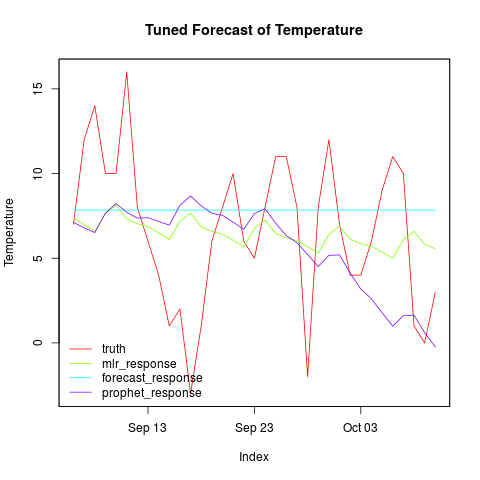
\includegraphics[width=\linewidth]{paper_figures/plot_ets_vs_forecast.png}
  \centering
  \caption{Forecasts of the tuned ETS from \pkg{mlr} and \pkg{forecast} and the GAM model from \pkg{prophet}}
  \label{fig:mlrvsforecast}
\end{figure}

\subsection{Tuning a GARCH model}

To this author's knowledge, this is the first package in \proglang{R} that allows for automated tuning and training of GARCH models~\cite{garchengels}. It is possible to pass and train multiple types of GARCH models while also tuning the model's respective parameters. In this example \code{predict.type = "quantile"} is used to estimate confidence intervals for the forecast.

\singlespacing
\begin{knitrout}
\definecolor{shadecolor}{rgb}{0.969, 0.969, 0.969}\color{fgcolor}\begin{kframe}
\begin{alltt}
\hlcom{# make resample description}
\hlstd{resampDesc} \hlkwb{=} \hlkwd{makeResampleDesc}\hlstd{(}\hlstr{"GrowingCV"}\hlstd{,} \hlkwc{horizon} \hlstd{=} \hlnum{35L}\hlstd{,}
                          \hlkwc{initial.window} \hlstd{=} \hlnum{.6}\hlstd{,}
                          \hlkwc{size} \hlstd{=} \hlkwd{nrow}\hlstd{(}\hlkwd{getTaskData}\hlstd{(climate.task)),}
                          \hlkwc{skip} \hlstd{=} \hlnum{.045}\hlstd{)}

\hlcom{# Make a tuning grid for GARCH}
\hlstd{par_set} \hlkwb{=} \hlkwd{makeParamSet}\hlstd{(}
  \hlkwd{makeDiscreteParam}\hlstd{(}\hlkwc{id} \hlstd{=} \hlstr{"model"}\hlstd{,}
                    \hlkwc{values} \hlstd{=} \hlkwd{c}\hlstd{(}\hlstr{"sGARCH"}\hlstd{,} \hlstr{"csGARCH"}\hlstd{)),}
  \hlkwd{makeIntegerVectorParam}\hlstd{(}\hlkwc{id} \hlstd{=} \hlstr{"garchOrder"}\hlstd{,} \hlkwc{len} \hlstd{=} \hlnum{2L}\hlstd{,}
                         \hlkwc{lower} \hlstd{=} \hlnum{1}\hlstd{,} \hlkwc{upper} \hlstd{=} \hlnum{4}\hlstd{),}
  \hlkwd{makeIntegerVectorParam}\hlstd{(}\hlkwc{id} \hlstd{=} \hlstr{"armaOrder"}\hlstd{,} \hlkwc{len} \hlstd{=} \hlnum{2L}\hlstd{,}
                         \hlkwc{lower} \hlstd{=} \hlnum{1}\hlstd{,} \hlkwc{upper} \hlstd{=} \hlnum{5}\hlstd{),}
  \hlkwd{makeLogicalParam}\hlstd{(}\hlkwc{id} \hlstd{=} \hlstr{"include.mean"}\hlstd{),}
  \hlkwd{makeLogicalParam}\hlstd{(}\hlkwc{id} \hlstd{=} \hlstr{"archm"}\hlstd{),}
  \hlkwd{makeDiscreteParam}\hlstd{(}\hlkwc{id} \hlstd{=} \hlstr{"distribution.model"}\hlstd{,}
                    \hlkwc{values} \hlstd{=} \hlkwd{c}\hlstd{(}\hlstr{"norm"}\hlstd{,}\hlstr{"std"}\hlstd{,}\hlstr{"jsu"}\hlstd{))}
\hlstd{)}

\hlcom{#Specify tune by F-racing}
\hlstd{ctrl} \hlkwb{=} \hlkwd{makeTuneControlIrace}\hlstd{(}\hlkwc{maxExperiments} \hlstd{=} \hlnum{300L}\hlstd{)}
\hlstd{garch.mod} \hlkwb{=} \hlkwd{makeLearner}\hlstd{(}\hlstr{"fcregr.garch"}\hlstd{,} \hlkwc{n.ahead}\hlstd{=} \hlnum{35}\hlstd{,} \hlkwc{solver} \hlstd{=} \hlstr{"hybrid"}\hlstd{)}
\hlcom{#Tuning in parallel}
\hlkwd{parallelStart}\hlstd{(}\hlstr{"multicore"}\hlstd{,}\hlnum{4}\hlstd{,} \hlkwc{level} \hlstd{=} \hlstr{"mlr.resample"}\hlstd{)}
\hlkwd{configureMlr}\hlstd{(}\hlkwc{on.learner.error} \hlstd{=} \hlstr{"warn"}\hlstd{)}
\hlkwd{set.seed}\hlstd{(}\hlnum{1234}\hlstd{)}
\hlstd{garchTune} \hlkwb{=} \hlkwd{tuneParams}\hlstd{(garch.mod,}
                    \hlkwc{task} \hlstd{= climate.task,} \hlkwc{resampling} \hlstd{= resampDesc,}
                    \hlkwc{par.set} \hlstd{= par_set,} \hlkwc{control} \hlstd{= ctrl,}
                    \hlkwc{measures} \hlstd{= mase)}
\hlkwd{parallelStop}\hlstd{()}
\hlstd{garchTune}\hlopt{$}\hlstd{y}
\end{alltt}
\end{kframe}
\end{knitrout}
\doublespacing



\begin{knitrout}
\definecolor{shadecolor}{rgb}{0.969, 0.969, 0.969}\color{fgcolor}\begin{kframe}
\begin{verbatim}
## mase.test.mean 
##      0.8949257
\end{verbatim}
\end{kframe}
\end{knitrout}


Because the partial dependence plots are still in development they do not work well with \code{makeNumericVectorParams()} such as \code{garchOrder} and \code{armaOrder}. Instead of looking at each $p,q$ individually, the sum of the coefficient values for the $p,q$ order of the GARCH component and the ARMA component are plotted.

\singlespacing


\begin{knitrout}
\definecolor{shadecolor}{rgb}{0.969, 0.969, 0.969}\color{fgcolor}\begin{kframe}
\begin{alltt}
\hlkwd{plotHyperParsEffect}\hlstd{(garch.hyperpar,} \hlkwc{x}\hlstd{=} \hlstr{"garchOrder"}\hlstd{,}
                    \hlkwc{y} \hlstd{=} \hlstr{"mase.test.mean"}\hlstd{,} \hlkwc{plot.type} \hlstd{=} \hlstr{"line"}\hlstd{,}
                     \hlkwc{partial.dep.learn} \hlstd{=} \hlstr{"regr.randomForest"}\hlstd{)}\hlopt{+}
  \hlkwd{theme_tufte}\hlstd{()} \hlopt{+}\hlkwd{theme}\hlstd{(}\hlkwc{text} \hlstd{=} \hlkwd{element_text}\hlstd{(}\hlkwc{size}\hlstd{=}\hlnum{20}\hlstd{))}
\hlkwd{plotHyperParsEffect}\hlstd{(garch.hyperpar,} \hlkwc{x}\hlstd{=} \hlstr{"armaOrder"}\hlstd{,}
                    \hlkwc{y} \hlstd{=} \hlstr{"mase.test.mean"}\hlstd{,} \hlkwc{plot.type} \hlstd{=} \hlstr{"line"}\hlstd{,}
                     \hlkwc{partial.dep.learn} \hlstd{=} \hlstr{"regr.randomForest"}\hlstd{)}\hlopt{+}
  \hlkwd{theme_tufte}\hlstd{()} \hlopt{+}\hlkwd{theme}\hlstd{(}\hlkwc{text} \hlstd{=} \hlkwd{element_text}\hlstd{(}\hlkwc{size}\hlstd{=}\hlnum{20}\hlstd{))}
\end{alltt}
\end{kframe}
\end{knitrout}



\begin{figure}[h!]
\centering
\begin{minipage}{.5\textwidth}
  \centering
  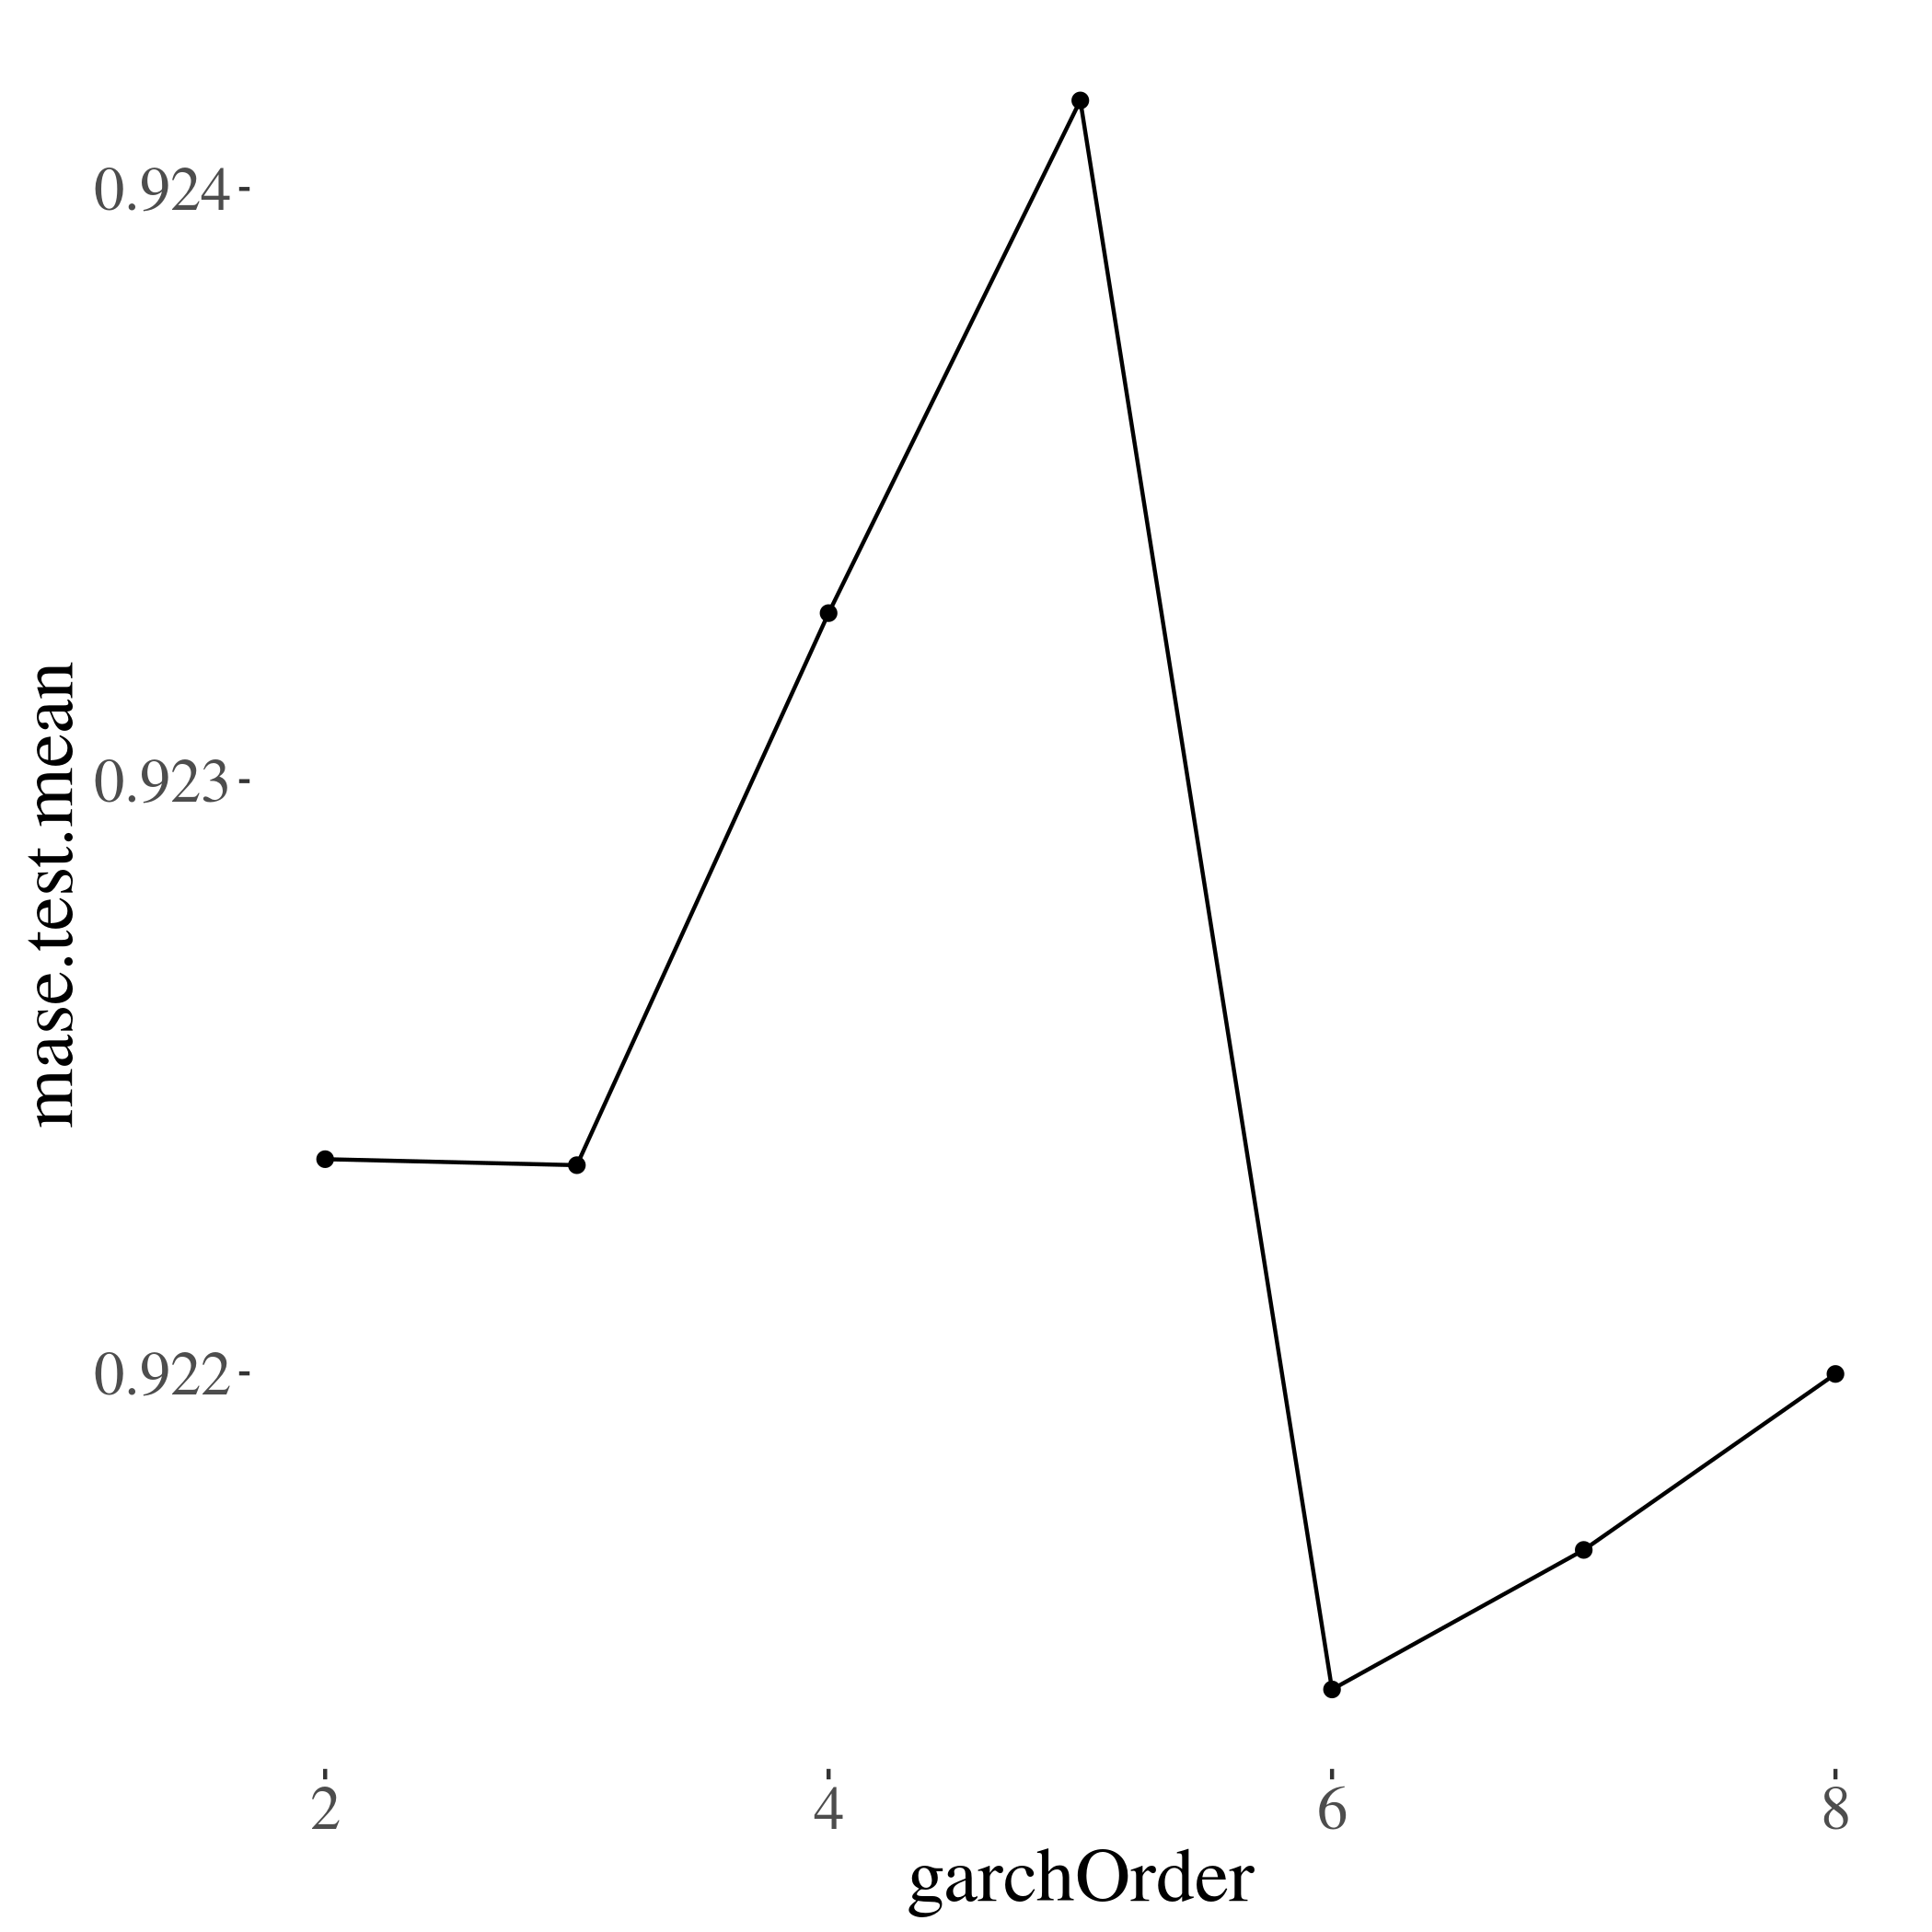
\includegraphics[width=\linewidth]{paper_figures/garch_order.png}
  \label{fig:test1}
\end{minipage}%
\begin{minipage}{.5\textwidth}
  \centering
  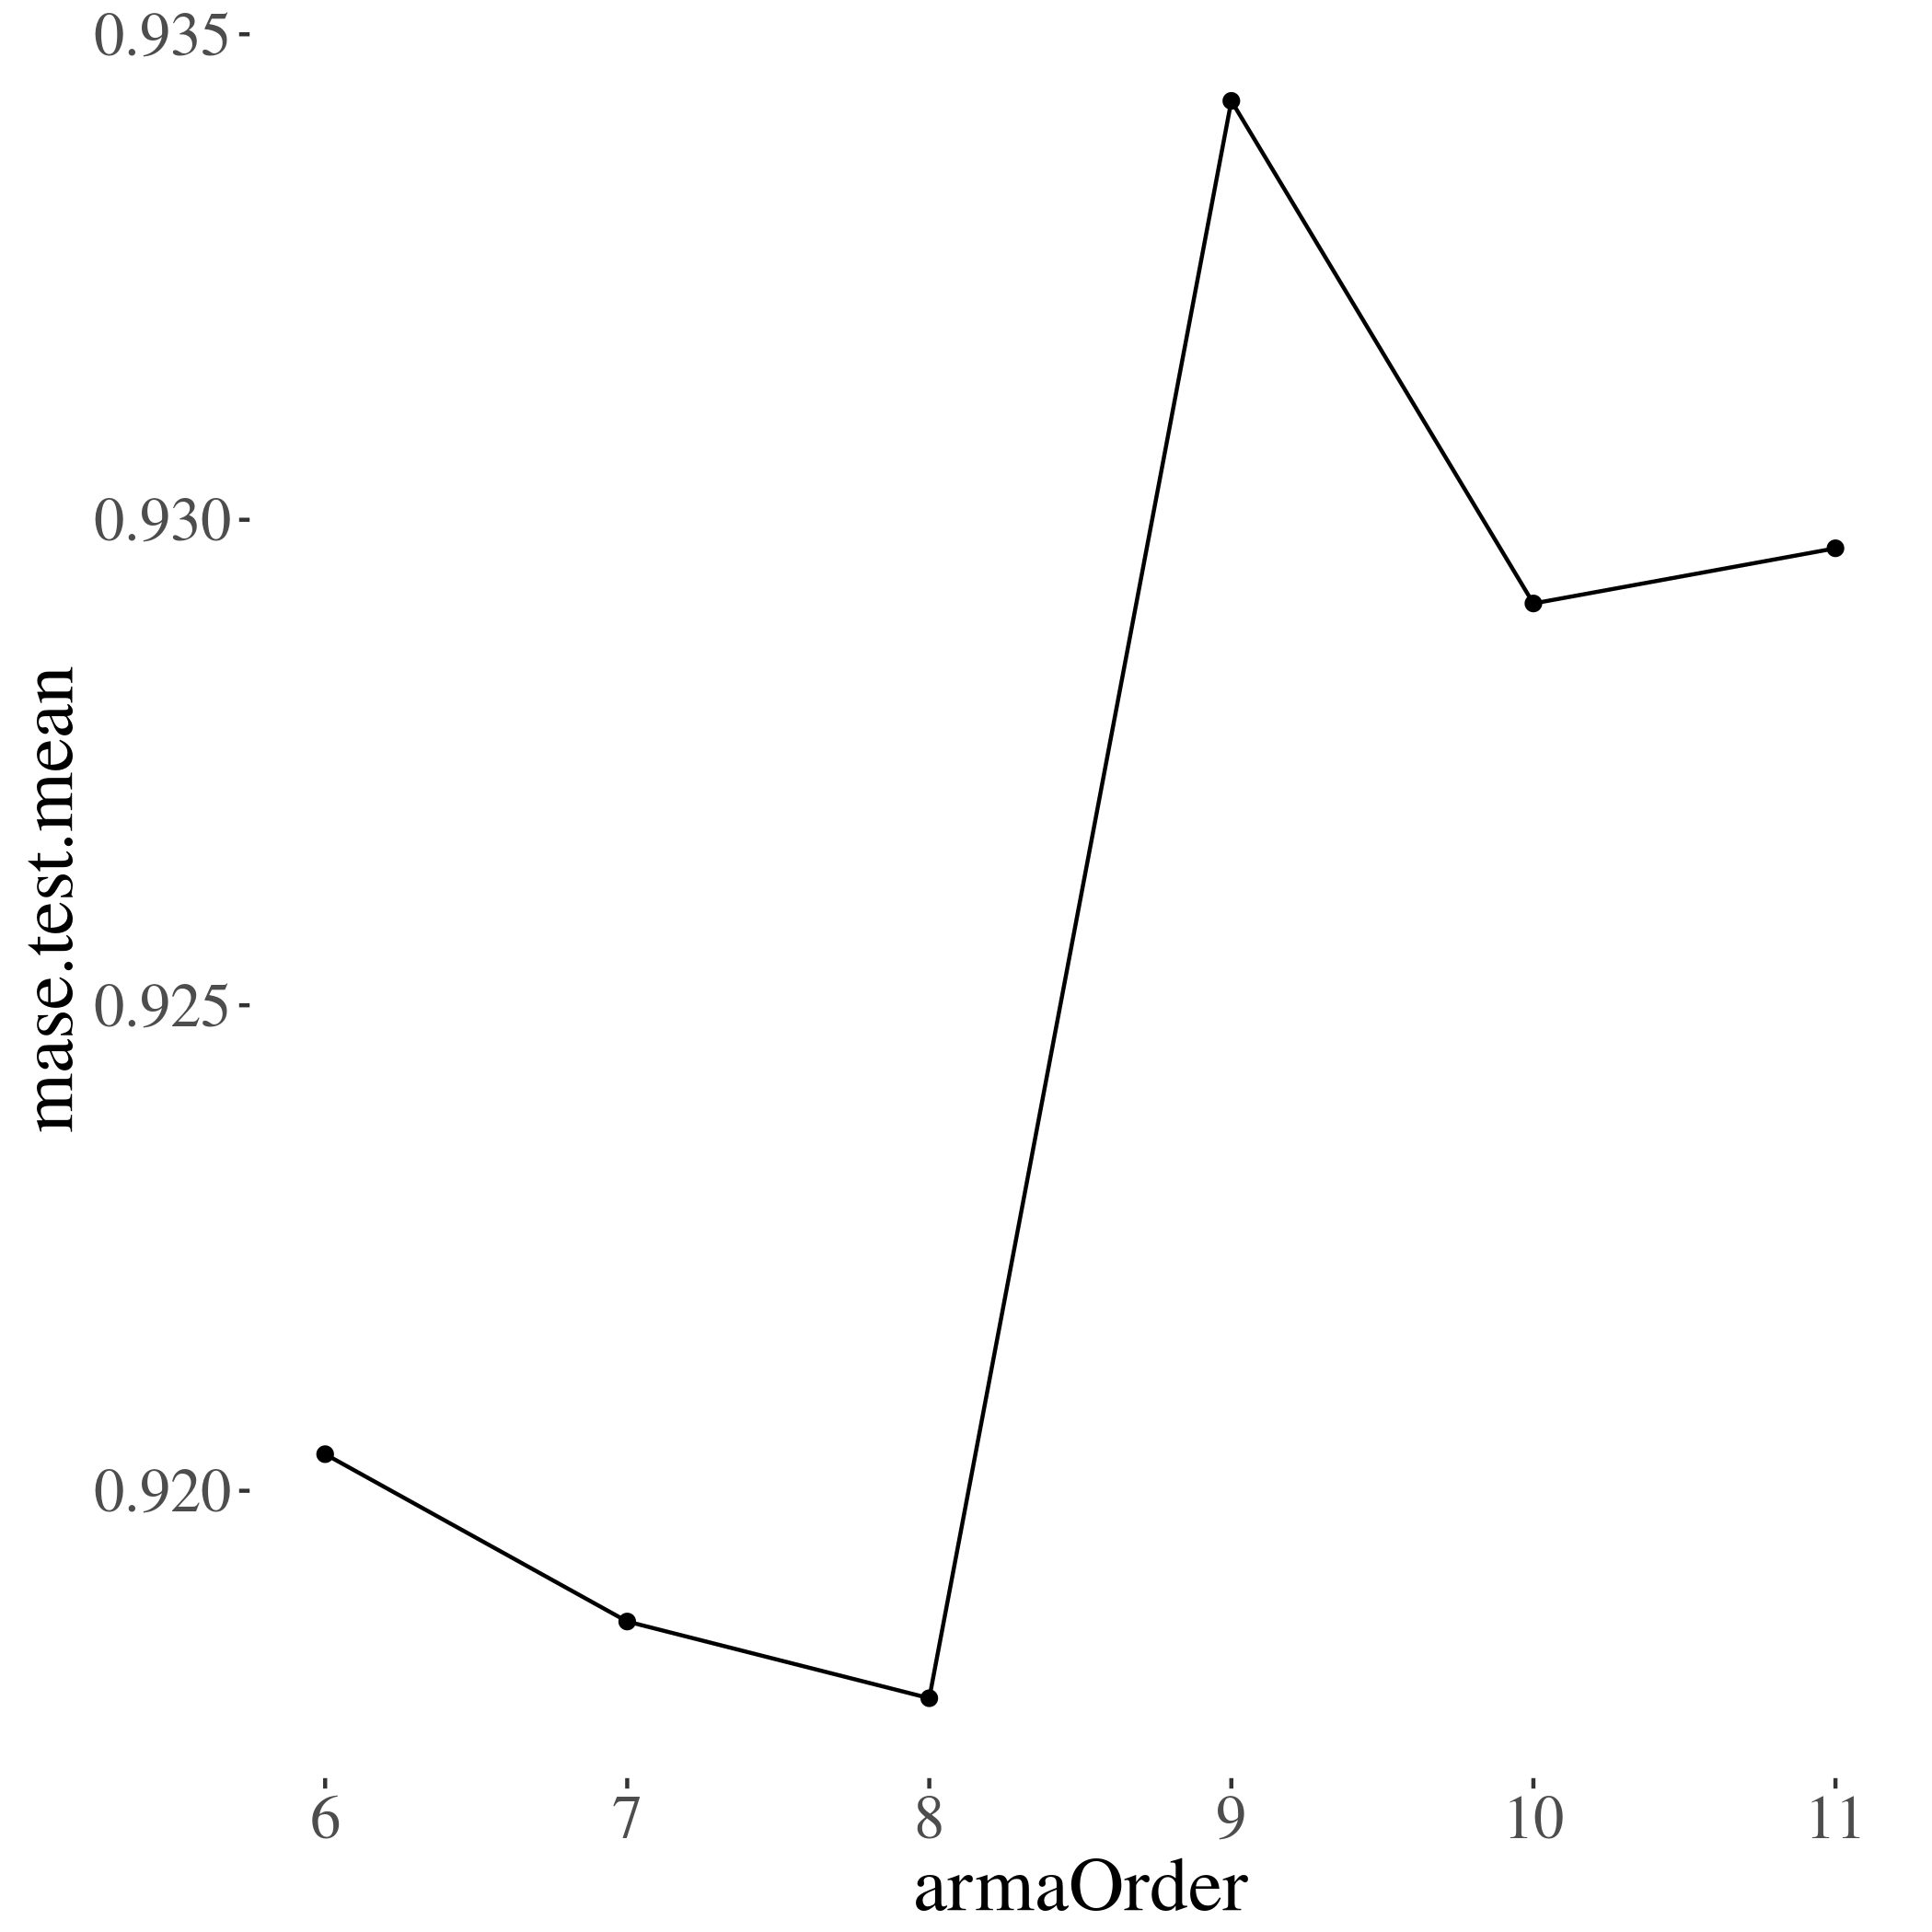
\includegraphics[width=\linewidth]{paper_figures/arma_order.png}
  \label{fig:test2}
\end{minipage}
\caption{The figure on the left shows the dependence of the MASE score averaged over all windows for each value of the sum of $p,q$ terms in the GARCH order. The figure on the right does the same, but for the ARMA order}
\label{fig:depGarch}
\end{figure}
\doublespacing

The dependence plots in figure~\ref{fig:depGarch} show that the best combinations of GARCH order are six and ARMA order is eight. The forecasting extension of \pkg{mlr} treats forecasting models with quantiles the same as any other learner post-tuning. The best hyperparameters are taken, and a final model trains over the entire dataset.

\singlespacing
\begin{knitrout}
\definecolor{shadecolor}{rgb}{0.969, 0.969, 0.969}\color{fgcolor}\begin{kframe}
\begin{alltt}
\hlcom{# Get the hyperpars and train the best GARCH model}
\hlstd{tuned.lrn} \hlkwb{=} \hlkwd{setHyperPars}\hlstd{(}\hlkwd{makeLearner}\hlstd{(}\hlstr{"fcregr.garch"}\hlstd{,}
                                     \hlkwc{predict.type} \hlstd{=} \hlstr{"quantile"}\hlstd{,}
                                     \hlkwc{n.ahead} \hlstd{=} \hlnum{35}\hlstd{),}
                         \hlkwc{par.vals} \hlstd{= garchTune}\hlopt{$}\hlstd{x)}
\hlstd{garch.train} \hlkwb{=} \hlkwd{train}\hlstd{(tuned.lrn, climate.task)}
\end{alltt}
\end{kframe}
\end{knitrout}


\begin{knitrout}
\definecolor{shadecolor}{rgb}{0.969, 0.969, 0.969}\color{fgcolor}\begin{kframe}
\begin{alltt}
\hlstd{climate.pred} \hlkwb{=} \hlkwd{predict}\hlstd{(garch.train,} \hlkwc{newdata} \hlstd{= m4.test)}
\hlstd{climate.pred}
\end{alltt}
\begin{verbatim}
## Prediction: 35 observations
## predict.type: quantile
## threshold: 
## time: 0.01
##            truth response se.quantile0.05 se.quantile0.95
## 2009-09-06     7 3.791806     -3.15797841        10.74159
## 2009-09-07    12 5.670953     -1.20007412        12.54198
## 2009-09-08    14 6.892649     -0.02135743        13.80666
## 2009-09-09    10 7.454873      0.55302644        14.35672
## 2009-09-10    10 7.752365      0.83784992        14.66688
## 2009-09-11    16 7.767169      0.85125791        14.68308
## ... (35 rows, 4 cols)
\end{verbatim}
\end{kframe}
\end{knitrout}



\begin{figure}[h!]
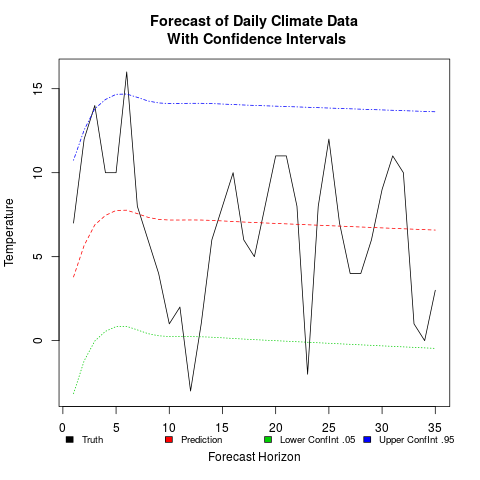
\includegraphics[width=\linewidth]{paper_figures/plot_garch_final.png}
\centering
\caption{The GARCH model with confidence intervals}
\label{fig:garch_final}
\end{figure}

\begin{knitrout}
\definecolor{shadecolor}{rgb}{0.969, 0.969, 0.969}\color{fgcolor}\begin{kframe}
\begin{alltt}
\hlkwd{performance}\hlstd{(climate.pred,} \hlkwc{measures} \hlstd{= mase,} \hlkwc{task} \hlstd{= climate.task)}
\end{alltt}
\begin{verbatim}
##      mase 
## 0.6663385
\end{verbatim}
\end{kframe}
\end{knitrout}

\doublespacing

The simple model here performs relatively well. Figure~\ref{fig:garch_final} shows that the extremes of the test data are almost all within the given bounds of the 95\% confidence interval. With a bit more tuning and perhaps an alternative control for the search over the parameter space, the reader would easily find a better model. While GARCH is excellent at catching the conditional heteroscedasticity of the past series, the ETS model performs well in its ability to catch additive and multiplicative factors of the time series. Section~\ref{sub:stackedUnivar} goes over how to stack forecasting models to make use of the best characteristics of each.


\section{Forecasting with Machine Learning Models}
\label{sec:preproc}
\subsection{Forecasting with Regression Tasks}
\label{sec:preprocAR}
\doublespacing
The forecasting extension of \pkg{mlr} includes a preprocessing function that allows forecasting with supervised machine learning models. The function \code{createLagDiffFeatures()} allows for $AR(p,d)$ structures to be embedded in machine learning models.
\singlespacing
\begin{knitrout}
\definecolor{shadecolor}{rgb}{0.969, 0.969, 0.969}\color{fgcolor}\begin{kframe}
\begin{alltt}
\hlstd{climate.regr.task} \hlkwb{=} \hlkwd{makeRegrTask}\hlstd{(}\hlkwc{id} \hlstd{=} \hlstr{"lagged gbm"}\hlstd{,}
                                 \hlkwc{data} \hlstd{=} \hlkwd{as.data.frame}\hlstd{(m4.train),}
                                 \hlkwc{target} \hlstd{=} \hlstr{"target_var"}\hlstd{)}
\hlstd{climate.task.lag} \hlkwb{=} \hlkwd{createLagDiffFeatures}\hlstd{(climate.regr.task,}
                                         \hlkwc{lag} \hlstd{=} \hlnum{1L}\hlopt{:}\hlnum{165L}\hlstd{,}
                                         \hlkwc{difference} \hlstd{=} \hlnum{0L}\hlstd{,}
                                         \hlkwc{na.pad}\hlstd{=}\hlnum{FALSE}\hlstd{)}
\hlstd{climate.task.lag}
\end{alltt}
\begin{verbatim}
## Supervised task: lagged gbm
## Type: regr
## Target: target_var
## Observations: 475
## Features:
## numerics  factors  ordered 
##      165        0        0 
## Missings: FALSE
## Has weights: FALSE
## Has blocking: FALSE
\end{verbatim}
\end{kframe}
\end{knitrout}
\doublespacing

Notice that \code{createLagDiffFeatures()} returns a new task with the lagged variables as the new features. Once the lagged task is created the model is trained or tuned like any other. The example below uses a gradient boosting machine~\cite{gbm} learner with an $AR(p,q)$ data generating process to forecast the M4 temperature data for 35 periods.

\singlespacing
\begin{knitrout}
\definecolor{shadecolor}{rgb}{0.969, 0.969, 0.969}\color{fgcolor}\begin{kframe}
\begin{alltt}
\hlcom{# make Gradient Boosting Machine}
\hlstd{lag.gbm} \hlkwb{=} \hlkwd{makeLearner}\hlstd{(}\hlstr{"regr.gbm"}\hlstd{,}
                      \hlkwc{par.vals} \hlstd{=} \hlkwd{list}\hlstd{(}\hlkwc{n.trees} \hlstd{=} \hlnum{20000}\hlstd{,}
                                      \hlkwc{shrinkage} \hlstd{=} \hlnum{.000001}\hlstd{,}
                                      \hlkwc{interaction.depth} \hlstd{=} \hlnum{16}\hlstd{,}
                                      \hlkwc{bag.fraction} \hlstd{=} \hlnum{.7}\hlstd{))}
\hlstd{gbm.train} \hlkwb{=} \hlkwd{train}\hlstd{(lag.gbm, climate.task.lag)}
\end{alltt}
\end{kframe}
\end{knitrout}





\doublespacing

The \code{forecast()} function allows machine learning models to do arbitrary n-step ahead forecasts. Let the one step ahead forecast be defined by

\begin{equation}
\hat{y}_{t+1} = \sum_{i=1}^p \left(\rho_i \Delta_d y_{i} + \epsilon_{i}\right)
\end{equation}
where $\rho_i$ is the autoregressive parameter of order $p$ and $d$ is the lag of the difference operator $\Delta$. Then the $n$-step ahead forecast is defined as

\begin{equation}
\hat{y}_{t+n} = \sum_{i=t+1}^{n} \left(\rho_i \Delta_d \hat{y}_{i} + \epsilon_{i}\right)
\end{equation}


\singlespacing
\begin{knitrout}
\definecolor{shadecolor}{rgb}{0.969, 0.969, 0.969}\color{fgcolor}\begin{kframe}
\begin{alltt}
\hlcom{# Forecast with GBM}
\hlstd{gbm.forecast} \hlkwb{=} \hlkwd{forecast}\hlstd{(gbm.train,} \hlkwc{h} \hlstd{=} \hlnum{35L}\hlstd{,}
                        \hlkwc{newdata} \hlstd{=} \hlkwd{as.data.frame}\hlstd{(m4.test))}
\end{alltt}
\end{kframe}
\end{knitrout}







\begin{knitrout}
\definecolor{shadecolor}{rgb}{0.969, 0.969, 0.969}\color{fgcolor}\begin{kframe}
\begin{alltt}
\hlstd{gbm.forecast}
\end{alltt}
\begin{verbatim}
## Prediction: 35 observations
## predict.type: response
## threshold: 
## time: 5.16
##   truth response
## 1     7 8.589142
## 2    12 8.645475
## 3    14 8.649393
## 4    10 8.651946
## 5    10 8.670011
## 6    16 8.655914
## ... (35 rows, 2 cols)
\end{verbatim}
\begin{alltt}
\hlkwd{performance}\hlstd{(}\hlkwc{pred} \hlstd{= gbm.forecast,}
            \hlkwc{measures} \hlstd{= mase,}
            \hlkwc{task} \hlstd{= climate.regr.task)}
\end{alltt}
\begin{verbatim}
##     mase 
## 1.061039
\end{verbatim}
\end{kframe}
\end{knitrout}

\doublespacing



\begin{figure}[h!]
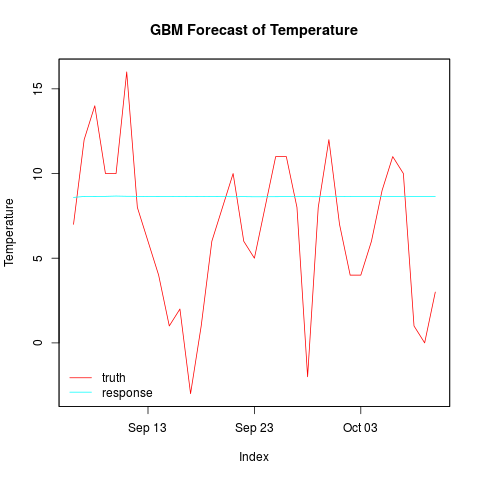
\includegraphics[width=.8\linewidth]{paper_figures/plot_gbm_fore.png}
\centering
\caption{The forecast of the M4 data using a Gradient Boosting Machine}
\label{fig:gbm_final}
\end{figure}

The forecasts in figure~\ref{fig:gbm_final} show the forecasts from the $AR(p,d)$ gradient boosting machine model. The autoregressive data generating process works for all regression machine learners which will allow researchers an easy haven for testing out machine learning models in the context of forecasting

%model placing the highest value on the most recent data. When the latest data is much more important than other past periods, this creates a weak decay scheme which causes forecasts to drift quickly to an average value.

\subsection{Forecasting with Classification Tasks}

Forecasting for binary or multiclass outcomes~\cite{forecastBinary} is a common problem in the real world. However, research in this area of forecasting only started picking up speed in the last decade~\cite{ElliotBinary}. The forecasting extension of \pkg{mlr} gives econometricians the ability to take all the classification models in \pkg{mlr} and apply them to the forecasting context. For developing trading strategies, there are usually a discrete set of choices such as to buy, sell, or hold onto a stock. The forecasting extension of \pkg{mlr} allows for classification models that forecast these options~\cite{foreclassif}. The code below implements a simple buy, sell, or hold trading strategy. If the stock goes up by 3\% over a 12 day period then a buy is executed, down 2\% a sell is executed, and otherwise no action will be taken. The probability of the best action being a buy, sell, or hold for the next 10 days of trades are then forecast using the adaboost algorithm~\cite{adaboost}. Data is divided into 1838 periods for training and 10 periods for evaluating the forecasting.

\singlespacing
\begin{knitrout}
\definecolor{shadecolor}{rgb}{0.969, 0.969, 0.969}\color{fgcolor}\begin{kframe}
\begin{alltt}
\hlcom{# Make Trading Strategy}
\hlstd{DAX} \hlkwb{=} \hlstd{EuStockMarkets}\hlopt{$}\hlstd{DAX}\hlopt{/}\hlkwd{lag}\hlstd{(EuStockMarkets}\hlopt{$}\hlstd{DAX,}
                             \hlnum{12}\hlstd{,}\hlkwc{na.pad} \hlstd{=} \hlnum{FALSE}\hlstd{)} \hlopt{-} \hlnum{1}
\hlstd{trade.strat} \hlkwb{=} \hlkwd{ifelse}\hlstd{(DAX} \hlopt{>} \hlnum{.03}\hlstd{,} \hlstr{"Buy"}\hlstd{,}
                     \hlkwd{ifelse}\hlstd{(DAX} \hlopt{< -}\hlnum{.02}\hlstd{,} \hlstr{"Sell"}\hlstd{,} \hlstr{"Hold"}\hlstd{))}
\hlstd{euro.classif.data} \hlkwb{=} \hlkwd{data.frame}\hlstd{(}\hlkwc{trade.strat} \hlstd{= trade.strat ,}
                               \hlkwc{row.names} \hlstd{=} \hlkwd{index}\hlstd{(trade.strat))}
\hlstd{euro.classif.train} \hlkwb{=} \hlstd{euro.classif.data[}\hlnum{1}\hlopt{:}\hlnum{1838}\hlstd{,,}\hlkwc{drop} \hlstd{=} \hlnum{FALSE}\hlstd{]}
\hlstd{euro.classif.test}  \hlkwb{=} \hlstd{euro.classif.data[}\hlnum{1839}\hlopt{:}\hlnum{1848}\hlstd{,,}\hlkwc{drop} \hlstd{=} \hlnum{FALSE}\hlstd{]}
\end{alltt}
\end{kframe}
\end{knitrout}



\begin{figure}[h!]
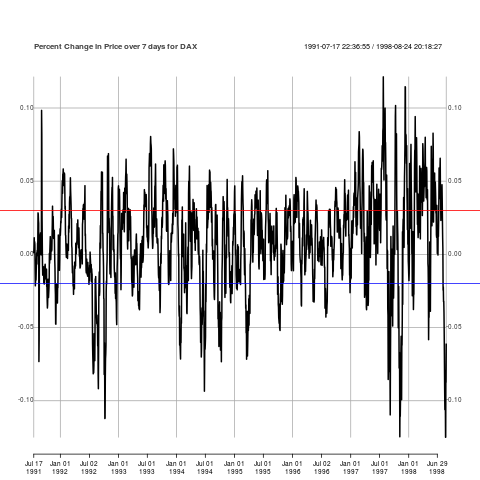
\includegraphics[width=\linewidth]{paper_figures/plot_classif_fore.png}
\centering
\caption{The percent change in price over a 7 day period for DAX. The top red line represents when a buy will be executed while the bottom blue line represents when a sell will be executed.}
\label{fig:classif_plot}
\end{figure}

\begin{knitrout}
\definecolor{shadecolor}{rgb}{0.969, 0.969, 0.969}\color{fgcolor}\begin{kframe}
\begin{alltt}
\hlstd{classif.task} \hlkwb{=} \hlkwd{makeClassifTask}\hlstd{(}\hlkwc{data} \hlstd{= euro.classif.train,}
                               \hlkwc{target} \hlstd{=} \hlstr{"DAX"}\hlstd{)}

\hlcom{# Make Lagged Task and Learner}
\hlstd{classif.task.lag} \hlkwb{=} \hlkwd{createLagDiffFeatures}\hlstd{(classif.task,}
                                         \hlkwc{lag} \hlstd{=} \hlnum{1L}\hlopt{:}\hlnum{565L}\hlstd{,}
                                         \hlkwc{na.pad} \hlstd{=} \hlnum{FALSE}\hlstd{)}
\hlstd{classif.learn} \hlkwb{=} \hlkwd{makeLearner}\hlstd{(}\hlstr{"classif.boosting"}\hlstd{,}
                            \hlkwc{mfinal} \hlstd{=} \hlnum{250}\hlstd{,} \hlkwc{minsplit} \hlstd{=} \hlnum{13}\hlstd{,}
                            \hlkwc{predict.type} \hlstd{=} \hlstr{"prob"}\hlstd{)}
\end{alltt}
\end{kframe}
\end{knitrout}

\begin{knitrout}
\definecolor{shadecolor}{rgb}{0.969, 0.969, 0.969}\color{fgcolor}\begin{kframe}
\begin{alltt}
\hlstd{classif.train} \hlkwb{=} \hlkwd{train}\hlstd{(classif.learn, classif.task.lag)}
\hlcom{# Tune threshold}
\hlstd{classif.pred} \hlkwb{=} \hlkwd{predict}\hlstd{(classif.train,} \hlkwc{task} \hlstd{= classif.task.lag)}
\hlstd{classif.pred.thresh} \hlkwb{=} \hlkwd{tuneThreshold}\hlstd{(}\hlkwc{pred} \hlstd{= classif.pred,}
                                    \hlkwc{measure} \hlstd{= multiclass.au1p)}
\hlstd{classif.train}\hlopt{$}\hlstd{learner}\hlopt{$}\hlstd{predict.threshold} \hlkwb{=} \hlstd{classif.pred.thresh}\hlopt{$}\hlstd{th}
\hlcom{# Forecast}
\hlstd{classif.fc} \hlkwb{=} \hlkwd{forecast}\hlstd{(classif.train,} \hlkwc{h}\hlstd{=}\hlnum{10}\hlstd{,}
                      \hlkwc{newdata} \hlstd{= euro.classif.test)}
\end{alltt}
\end{kframe}
\end{knitrout}





\begin{knitrout}
\definecolor{shadecolor}{rgb}{0.969, 0.969, 0.969}\color{fgcolor}\begin{kframe}
\begin{alltt}
\hlstd{classif.fc}
\end{alltt}
\begin{verbatim}
## Prediction: 10 observations
## predict.type: prob
## threshold: Buy=0.21,Hold=0.26,Sell=0.53
## time: 363.49
##   truth    prob.Buy prob.Hold prob.Sell response
## 1  Sell 0.004166354 0.3657509 0.6300828     Hold
## 2  Sell 0.173724131 0.4937166 0.3325592     Hold
## 3  Sell 0.205848370 0.4950168 0.2991349     Hold
## 4  Sell 0.162088380 0.4725685 0.3653431     Hold
## 5  Sell 0.236698547 0.4706002 0.2927012     Hold
## 6  Sell 0.176916303 0.5389581 0.2841256     Hold
## ... (10 rows, 5 cols)
\end{verbatim}
\begin{alltt}
\hlkwd{performance}\hlstd{(classif.fc)}
\end{alltt}
\begin{verbatim}
## mmce 
##    1
\end{verbatim}
\end{kframe}
\end{knitrout}
\doublespacing

It is obvious that an MMCE of zero should be looked at with incredulousness. It can be seen in figure~\ref{fig:classif_plot} that the last periods before the test data are all below the rule to execute a sell and so the model follows the trend. Further testing is necessary with multiple types of data and models to assess the usefullness of forecasting classification within \pkg{mlr}. With the models and methodologies available in \pkg{mlr}, forecasting binary or multiclass outcomes is now as simple as utilizing any other machine learning model. These tools can allow for further research in areas such as forecasting directions of stock movement~\cite{markClassifStock} and extreme values~\cite{Chen2015UsingEV}.

\section{Lambert W Transforms}
\label{sec:lambert}
Many machine learning and time series models rely on the assumption that the data or errors fit a normal distribution. This assumption becomes precarious when modeling the asymmetric and fat-tailed data of the real world. Lambert $W\times F_X$ transforms are a family of generalized skewed distributions~\cite{LambertGeneral} that have bijective and parametric functions that allow heavy tailed and asymmetric data to appear more Gaussian~\cite{GaussLam}.

Let $U$ be a continuous random variable with cdf $F_U(u|\beta)$ and pdf $f_U(u|\beta)$ given $\beta$ is a parameter vector. Define a continuous location-scale random variable $X\sim F_X(x|\beta)$. A location-scale skewed Lambert $W\times F_X$ random variable is defined as

\begin{equation}
Z = U\exp \left(\frac{\delta}{2} (U^2)\right),\; \delta\ge 0
\label{eq:hdist}
\end{equation}

And the heavy-tailed Lambert $W\times F_X$ random variable can be defined as

\begin{equation}
Z = U\exp\left(\frac{\delta}{2}(U^2)^\alpha\right),\; \delta\ge 0\; \alpha > 0
\label{eq:hhdist2}
\end{equation}

Given that $U = (X-\mu_X)/\sigma_X$ where $\mu_X$, $\sigma_X$, $\delta$, and $\alpha$ are the mean and standard deviation of X and the parameters to control skewness and asymmetry , respectively. When $\delta = 0$, equation~\ref{eq:hdist} reduces to a standard normal distribution. Equation~\ref{eq:hhdist2} is the general form of Tukey's $h$ distribution~\cite{ghdist} and the basis for Morgenthaler and Tukey's~\cite{hhdist} skewed, heavy tailed family of $hh$ random variables.

\begin{equation}
  Z = \begin{cases}
               U\exp\left(\frac{\delta_l}{2}(U^2)^\alpha_l\right),\; \delta_l \ge 0\; \alpha_l > 0\\
               U\exp\left(\frac{\delta_r}{2}(U^2)^\alpha_r\right),\; \delta_r \ge 0 \alpha_r > 0
            \end{cases}
\end{equation}

\singlespacing


\begin{figure}[H]

\includegraphics[width=\linewidth]{paper_figures/cauchy_h_train.png}
\centering
\caption{The top plot are samples from the cauchy distribution where the bottom plot represents the cauchy transformed variables with the $hh$ distribution to make the samples approximately normal.}
\label{fig:cauchy_lambert}
\end{figure}

\doublespacing

The function \code{Gaussianize()} is available in the package \pkg{LambertW} and has been made into a preprocessing function in \pkg{mlr}. Instead of calling \code{makeLearner()} to create a model, the function \code{makePreprocWrapperLambert()} can be used to create the model. This means the pre-processing scheme integrates into the model. Integrating the pre-processing scheme directly on top of the model stops users from accidentally biasing their models due to improperly applying pre-processing. For instance, if a user demeaned their entire data set and then split the data into train and test subsets, the training data will be biased because demeaning the model over both the train and test data gives the training data information about the mean of the test data. What should happen instead is, the user first splits the data into training and test data, and then demeans each separately. Similarly, cross-validation follows the above scheme whereby each cross-validation will be biased if the user demeaned all of the training data at one time. It is very easy for a user, who assumes they have made a good faith attempt not to bias their model, to receive overconfident results. Embedding the pre-processing itself allows \pkg{mlr} to overcome this.

The pre-processing scheme is broken down into two main components. One function to gather and estimate necessary parameters in the training data, then a function to apply the learned preprocess over the training and test data. In the context of Lambert $W\times F_X$ transforms, the estimates for the parameters of the $h$, $hh$, or $s$ distribution that gaussianizes the data comes from the training data. Then the estimated parameter values from the training set are used during prediction to gaussianize the test observations. The code below follows this methodology, creating the model with Lambert preprocessing, training the model, and then performing prediction. The result to the user appears the same, but there is a significant reduction of bias in the background.

\singlespacing
\begin{knitrout}
\definecolor{shadecolor}{rgb}{0.969, 0.969, 0.969}\color{fgcolor}\begin{kframe}
\begin{alltt}
\hlcom{# Make a Learner with Lambert WxF() learner}
\hlstd{lamb.lrn} \hlkwb{=} \hlkwd{makePreprocWrapperLambert}\hlstd{(}\hlstr{"classif.lda"}\hlstd{,} \hlkwc{type} \hlstd{=} \hlstr{"s"}\hlstd{)}
\hlstd{lamb.lrn}
\end{alltt}
\begin{verbatim}
## Learner classif.lda.preproc from package MASS
## Type: classif
## Name: ; Short name: 
## Class: PreprocWrapperLambert
## Properties: numerics,factors,prob,twoclass,multiclass
## Predict-Type: response
## Hyperparameters: type=s,methods=IGMM,verbose=FALSE
\end{verbatim}
\begin{alltt}
\hlstd{lamb.trn} \hlkwb{=} \hlkwd{train}\hlstd{(lamb.lrn,iris.task,} \hlkwc{subset} \hlstd{=} \hlnum{1}\hlopt{:}\hlnum{120}\hlstd{)}
\hlstd{lamb.pred} \hlkwb{=} \hlkwd{predict}\hlstd{(lamb.trn, iris.task,} \hlkwc{subset} \hlstd{=} \hlnum{121}\hlopt{:}\hlnum{150}\hlstd{)}

\hlcom{# Do the non-LW version}
\hlstd{trn} \hlkwb{=} \hlkwd{train}\hlstd{(}\hlkwd{makeLearner}\hlstd{(}\hlstr{"classif.lda"}\hlstd{),iris.task,} \hlkwc{subset} \hlstd{=} \hlnum{1}\hlopt{:}\hlnum{120}\hlstd{)}
\hlstd{pred} \hlkwb{=} \hlkwd{predict}\hlstd{(trn, iris.task,} \hlkwc{subset} \hlstd{=} \hlnum{121}\hlopt{:}\hlnum{150}\hlstd{)}
\hlkwd{performance}\hlstd{(lamb.pred)}
\end{alltt}
\begin{verbatim}
##       mmce 
## 0.06666667
\end{verbatim}
\begin{alltt}
\hlkwd{performance}\hlstd{(pred)}
\end{alltt}
\begin{verbatim}
## mmce 
##  0.1
\end{verbatim}
\end{kframe}
\end{knitrout}
\doublespacing

\section{Stacking Forecasting Learners}
\label{sec:stackfore}
Stacking is a form of ensemble learning~\cite{ensembleOverview} in which a learning algorithm trains on the predictions of several other learning algorithms. Let $\tilde{y}_{i,m}$ be the prediction at time $i$ of model $m$. Given an aggregation function $\phi$, a stacked forecast learner~\cite{combineForecast} is represented as

\begin{equation}
\tilde{y}_{i+1} = \phi(\tilde{y}_{i+1,1}, \tilde{y}_{i+1,2},\dots, \tilde{y}_{i+1,m}, \sum_{j=1}^m \epsilon_{i+1,j})
\label{eq:ensemble}
\end{equation}

For a simple $\phi()$ such as the ensemble average, equation~\ref{eq:ensemble} becomes

\begin{equation}
\tilde{y}_{i+1} = \frac{\tilde{y}_{i+1,1} + \tilde{y}_{i+1,2} +\dots + \tilde{y}_{i+1,m}}{m}
\label{eq:ensembleAverage}
\end{equation}

In section~\ref{sub:stackedUnivar} the simple model average is used to show how stacked forecast models are built in \pkg{mlr}. Section~\ref{sub:multiStack} does a more advanced method of ensemble averaging involving the forecast of endogenous variables.

\subsection{Stacking Univariate Learners}
\label{sub:stackedUnivar}

For this example, the models TBATS, GARCH, and ARFIMA~\cite{arfima} are stacked together and averaged on the climate task data. A resample description is made, and the function \code{makeLearners()} is used to start many learners at the same time.

\singlespacing
\begin{knitrout}
\definecolor{shadecolor}{rgb}{0.969, 0.969, 0.969}\color{fgcolor}\begin{kframe}
\begin{alltt}
\hlstd{resamp.sub} \hlkwb{=} \hlkwd{makeResampleDesc}\hlstd{(}\hlstr{"GrowingCV"}\hlstd{,}
                          \hlkwc{horizon} \hlstd{=} \hlnum{35L}\hlstd{,}
                          \hlkwc{initial.window} \hlstd{=} \hlnum{.80}\hlstd{,}
                          \hlkwc{size} \hlstd{=} \hlkwd{nrow}\hlstd{(}\hlkwd{getTaskData}\hlstd{(climate.task)),}
                          \hlkwc{skip} \hlstd{=} \hlnum{.012}
                          \hlstd{)}
\hlstd{lrns} \hlkwb{=} \hlkwd{makeLearners}\hlstd{(}\hlkwd{c}\hlstd{(}\hlstr{"fcregr.tbats"}\hlstd{,}\hlstr{"fcregr.garch"}\hlstd{,}
                      \hlstr{"fcregr.arfima"}\hlstd{))}
\end{alltt}
\end{kframe}
\end{knitrout}
\doublespacing

The function \code{makeStackedLearner()} takes the initialized learners and sets the meta information for stacking. This method uses simple model averaging such as equation~\ref{eq:ensembleAverage}, however a super learner~\cite{Wolpert92stackedgeneralization} can be used here, where $\phi()$ becomes another machine learning model.

\singlespacing
\begin{knitrout}
\definecolor{shadecolor}{rgb}{0.969, 0.969, 0.969}\color{fgcolor}\begin{kframe}
\begin{alltt}
\hlstd{stack.forecast} \hlkwb{=} \hlkwd{makeStackedLearner}\hlstd{(}\hlkwc{base.learners} \hlstd{= lrns,}
                       \hlkwc{predict.type} \hlstd{=} \hlstr{"response"}\hlstd{,}
                       \hlkwc{method} \hlstd{=} \hlstr{"average"}\hlstd{)}
\end{alltt}
\end{kframe}
\end{knitrout}
\doublespacing

Each of the stacked learners are tuned over the cross product of all model parameters. This leads to a change in design where, given that some models may have the same argument names, the full name of the model is placed before the argument. Training over the cross-product of the model parameters leads to longer code, but it allows for a more honest perspective of how each model interacts in the stack.

\singlespacing
\begin{knitrout}
\definecolor{shadecolor}{rgb}{0.969, 0.969, 0.969}\color{fgcolor}\begin{kframe}
\begin{alltt}
\hlcom{# Simple param set for tuning sub learners}
\hlstd{ps} \hlkwb{=} \hlkwd{makeParamSet}\hlstd{(}
  \hlkwd{makeDiscreteParam}\hlstd{(}\hlstr{"fcregr.tbats.h"}\hlstd{,} \hlkwc{values} \hlstd{=} \hlnum{35}\hlstd{),}
  \hlkwd{makeDiscreteParam}\hlstd{(}\hlstr{"fcregr.garch.n.ahead"}\hlstd{,} \hlkwc{values} \hlstd{=} \hlnum{35}\hlstd{),}
  \hlkwd{makeDiscreteParam}\hlstd{(}\hlstr{"fcregr.arfima.h"}\hlstd{,} \hlkwc{values} \hlstd{=} \hlnum{35}\hlstd{),}
  \hlkwd{makeDiscreteParam}\hlstd{(}\hlstr{"fcregr.arfima.estim"}\hlstd{,} \hlkwc{values} \hlstd{=} \hlstr{"ls"}\hlstd{),}
  \hlkwd{makeDiscreteParam}\hlstd{(}\hlkwc{id} \hlstd{=} \hlstr{"fcregr.garch.model"}\hlstd{,}
                    \hlkwc{values} \hlstd{=} \hlkwd{c}\hlstd{(}\hlstr{"csGARCH"}\hlstd{)),}
  \hlkwd{makeIntegerVectorParam}\hlstd{(}\hlkwc{id} \hlstd{=} \hlstr{"fcregr.garch.garchOrder"}\hlstd{,}
                         \hlkwc{len} \hlstd{=} \hlnum{2L}\hlstd{,} \hlkwc{lower} \hlstd{=} \hlkwd{c}\hlstd{(}\hlnum{1}\hlstd{),}
                         \hlkwc{upper} \hlstd{=} \hlkwd{c}\hlstd{(}\hlnum{6}\hlstd{)),}
  \hlkwd{makeIntegerVectorParam}\hlstd{(}\hlkwc{id} \hlstd{=} \hlstr{"fcregr.garch.armaOrder"}\hlstd{,}
                         \hlkwc{len} \hlstd{=} \hlnum{2L}\hlstd{,} \hlkwc{lower} \hlstd{=} \hlkwd{c}\hlstd{(}\hlnum{1}\hlstd{),}
                         \hlkwc{upper} \hlstd{=} \hlkwd{c}\hlstd{(}\hlnum{4}\hlstd{)),}
  \hlkwd{makeDiscreteParam}\hlstd{(}\hlkwc{id} \hlstd{=} \hlstr{"fcregr.garch.distribution.model"}\hlstd{,}
                    \hlkwc{values} \hlstd{=} \hlkwd{c}\hlstd{(}\hlstr{"norm"}\hlstd{,}\hlstr{"std"}\hlstd{,}\hlstr{"jsu"}\hlstd{)),}
  \hlkwd{makeDiscreteParam}\hlstd{(}\hlstr{"fcregr.tbats.test"}\hlstd{,}
                    \hlkwc{values} \hlstd{=} \hlkwd{c}\hlstd{(}\hlstr{"kpss"}\hlstd{,}\hlstr{"adf"}\hlstd{,}\hlstr{"pp"}\hlstd{)),}
  \hlkwd{makeIntegerParam}\hlstd{(}\hlstr{"fcregr.tbats.max.P"}\hlstd{,} \hlkwc{lower} \hlstd{=} \hlnum{0}\hlstd{,} \hlkwc{upper} \hlstd{=} \hlnum{3}\hlstd{),}
  \hlkwd{makeIntegerParam}\hlstd{(}\hlstr{"fcregr.tbats.max.Q"}\hlstd{,} \hlkwc{lower} \hlstd{=} \hlnum{0}\hlstd{,} \hlkwc{upper} \hlstd{=} \hlnum{2}\hlstd{)}
\hlstd{)}
\hlstd{ctrl} \hlkwb{=} \hlkwd{makeTuneControlIrace}\hlstd{(}\hlkwc{maxExperiments} \hlstd{=} \hlnum{400L}\hlstd{)}
\hlcom{## tuning}
\hlkwd{library}\hlstd{(parallelMap)}
\hlkwd{parallelStart}\hlstd{(}\hlstr{"multicore"}\hlstd{,}\hlnum{8}\hlstd{)}
\hlkwd{configureMlr}\hlstd{(}\hlkwc{on.learner.error} \hlstd{=} \hlstr{"warn"}\hlstd{)}
\hlkwd{set.seed}\hlstd{(}\hlnum{1234}\hlstd{)}
\hlstd{fore.tune} \hlkwb{=} \hlkwd{tuneParams}\hlstd{(stack.forecast, climate.task,}
                       \hlkwc{resampling} \hlstd{= resamp.sub,}
                       \hlkwc{par.set} \hlstd{= ps,} \hlkwc{control} \hlstd{= ctrl,}
                       \hlkwc{measures} \hlstd{= mase,} \hlkwc{show.info} \hlstd{=} \hlnum{FALSE}\hlstd{)}
\hlkwd{parallelStop}\hlstd{()}
\end{alltt}
\end{kframe}
\end{knitrout}





\doublespacing

The rest of the modeling process flows in a way similar to the standard training and predicting schema. The function \code{setHyperPars2()} takes the best parameter models from the tuning process and assigns it to the final model to train over all of the data. Training and prediction operate in the same manner as univariate forecasters.

\singlespacing
\begin{knitrout}
\definecolor{shadecolor}{rgb}{0.969, 0.969, 0.969}\color{fgcolor}\begin{kframe}
\begin{alltt}
\hlcom{# get hyper params}
\hlstd{stack.forecast.tune}  \hlkwb{=} \hlkwd{setHyperPars2}\hlstd{(stack.forecast,fore.tune}\hlopt{$}\hlstd{x)}
\hlcom{# Train the final best models and predict}
\hlstd{stack.forecast.mod} \hlkwb{=} \hlkwd{train}\hlstd{(stack.forecast.tune,climate.task)}
\hlstd{stack.forecast.pred} \hlkwb{=} \hlkwd{predict}\hlstd{(stack.forecast.mod,}
                              \hlkwc{newdata} \hlstd{= m4.test)}
\hlstd{stack.forecast.pred}
\end{alltt}
\begin{verbatim}
## Prediction: 35 observations
## predict.type: response
## threshold: 
## time: 0.00
##            truth response
## 2009-09-06     7 4.818912
## 2009-09-07    12 6.996888
## 2009-09-08    14 7.721830
## 2009-09-09    10 7.918169
## 2009-09-10    10 7.880900
## 2009-09-11    16 8.030308
## ... (35 rows, 2 cols)
\end{verbatim}
\begin{alltt}
\hlkwd{performance}\hlstd{(stack.forecast.pred,mase,climate.task)}
\end{alltt}
\begin{verbatim}
##     mase 
## 0.722316
\end{verbatim}
\end{kframe}
\end{knitrout}



\begin{figure}[h!]
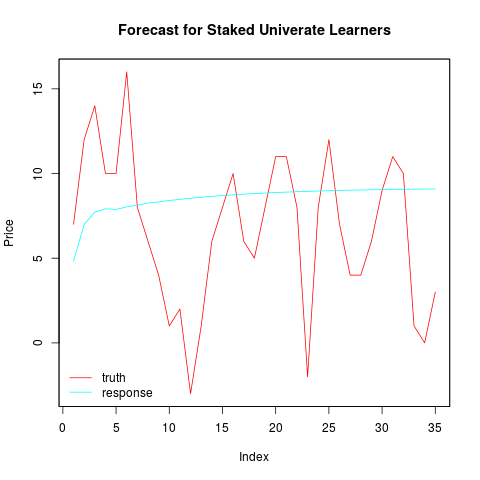
\includegraphics[width=\linewidth]{paper_figures/ensemble_pred.png}
\centering
\caption{The forecast of the M4 data using the Stacked ARFIMA, TBATS, and GARCH model}
\label{fig:ensemble_final}
\end{figure}

\doublespacing

\subsection{Multivariate Stacked Learner}
\label{sub:multiStack}

When there is a single target variable with multiple predictors, stacked learning can be used with multivariate forecasters to forecast the predictors and have a machine learning model train over the forecasts of all variables. For this, equation~\ref{eq:ensemble} can be modified to include forecasts of other predictors $x_{i,k}$ where $k$ is the index for each predictor variable

\begin{equation}
\tilde{y}_{i+1} = \phi(\tilde{y}_{i+1,1},\dots, \tilde{y}_{i+1,m}, \tilde{x}_{i+1,1},\dots, \tilde{x}_{i+1,k}, \sum_{j=1}^m \epsilon_{i+1,j}, \sum_{j=1}^k \epsilon_{i+1,j})
\label{eq:ensembleMulti}
\end{equation}

In the example below, a boosted glm~\cite{glmboost} is used as a super learner over a sparse lag multivariate VAR model to forecast FTSE prices. A resampling strategy is creating for both the underlying stacked learner and the super learner.

\singlespacing
\begin{knitrout}
\definecolor{shadecolor}{rgb}{0.969, 0.969, 0.969}\color{fgcolor}\begin{kframe}
\begin{alltt}
\hlstd{multfore.task} \hlkwb{=} \hlkwd{makeMultiForecastRegrTask}\hlstd{(}\hlkwc{id} \hlstd{=} \hlstr{"bigvar"}\hlstd{,}
                                          \hlkwc{data} \hlstd{= eu.train,}
                                          \hlkwc{target} \hlstd{=} \hlstr{"FTSE"}\hlstd{)}

\hlstd{resamp.sub} \hlkwb{=} \hlkwd{makeResampleDesc}\hlstd{(}\hlstr{"GrowingCV"}\hlstd{,}
                          \hlkwc{horizon} \hlstd{=} \hlnum{32L}\hlstd{,}
                          \hlkwc{initial.window} \hlstd{=} \hlnum{.90}\hlstd{,}
                          \hlkwc{size} \hlstd{=} \hlkwd{nrow}\hlstd{(}\hlkwd{getTaskData}\hlstd{(multfore.task)),}
                          \hlkwc{skip} \hlstd{=} \hlnum{.03}\hlstd{)}

\hlstd{resamp.super} \hlkwb{=} \hlkwd{makeResampleDesc}\hlstd{(}\hlstr{"CV"}\hlstd{,} \hlkwc{iters} \hlstd{=} \hlnum{3}\hlstd{)}
\end{alltt}
\end{kframe}
\end{knitrout}
\doublespacing

In \code{makeStackedLearner()}, the super learner argument contains the boosted glm model.

\singlespacing
\begin{knitrout}
\definecolor{shadecolor}{rgb}{0.969, 0.969, 0.969}\color{fgcolor}\begin{kframe}
\begin{alltt}
\hlstd{base} \hlkwb{=} \hlkwd{c}\hlstd{(}\hlstr{"mfcregr.BigVAR"}\hlstd{)}
\hlstd{lrns} \hlkwb{=} \hlkwd{lapply}\hlstd{(base, makeLearner)}
\hlstd{lrns} \hlkwb{=} \hlkwd{lapply}\hlstd{(lrns, setPredictType,} \hlstr{"response"}\hlstd{)}
\hlstd{lrns[[}\hlnum{1}\hlstd{]]}\hlopt{$}\hlstd{par.vals}\hlopt{$}\hlstd{verbose} \hlkwb{=} \hlnum{FALSE}
\hlstd{lrns[[}\hlnum{1}\hlstd{]]}\hlopt{$}\hlstd{par.vals}\hlopt{$}\hlstd{recursive} \hlkwb{=} \hlnum{FALSE}
\hlstd{lrns[[}\hlnum{1}\hlstd{]]}\hlopt{$}\hlstd{par.vals}\hlopt{$}\hlstd{struct} \hlkwb{=} \hlstr{"SparseLag"}


\hlstd{stack.forecast} \hlkwb{=} \hlkwd{makeStackedLearner}\hlstd{(}\hlkwc{base.learners} \hlstd{= lrns,}
                    \hlkwc{predict.type} \hlstd{=} \hlstr{"response"}\hlstd{,}
                    \hlkwc{super.learner} \hlstd{=} \hlkwd{makeLearner}\hlstd{(}\hlstr{"regr.glmboost"}\hlstd{,}
                                            \hlkwc{family} \hlstd{=} \hlstr{"Laplace"}\hlstd{),}
                    \hlkwc{method} \hlstd{=} \hlstr{"growing.cv"}\hlstd{,}
                    \hlkwc{resampling} \hlstd{= resamp.sub)}
\end{alltt}
\end{kframe}
\end{knitrout}
\doublespacing

Just as with univariate stacked forecasting models, a parameter set is created for the multivariate VAR model and tuning is done with \code{tuneParams()}.

\singlespacing
\begin{knitrout}
\definecolor{shadecolor}{rgb}{0.969, 0.969, 0.969}\color{fgcolor}\begin{kframe}
\begin{alltt}
\hlstd{ps} \hlkwb{=} \hlkwd{makeParamSet}\hlstd{(}
  \hlkwd{makeDiscreteParam}\hlstd{(}\hlstr{"mfcregr.BigVAR.p"}\hlstd{,} \hlkwc{values} \hlstd{=} \hlnum{9}\hlstd{),}
  \hlkwd{makeNumericVectorParam}\hlstd{(}\hlstr{"mfcregr.BigVAR.gran"}\hlstd{,} \hlkwc{len} \hlstd{=} \hlnum{2L}\hlstd{,}
                         \hlkwc{lower} \hlstd{=} \hlnum{30}\hlstd{,} \hlkwc{upper} \hlstd{=} \hlnum{40}\hlstd{),}
  \hlkwd{makeDiscreteParam}\hlstd{(}\hlstr{"mfcregr.BigVAR.h"}\hlstd{,} \hlkwc{values} \hlstd{=} \hlnum{32}\hlstd{),}
  \hlkwd{makeDiscreteParam}\hlstd{(}\hlstr{"mfcregr.BigVAR.n.ahead"}\hlstd{,} \hlkwc{values} \hlstd{=} \hlnum{32}\hlstd{)}
\hlstd{)}
  \hlcom{## tuning}
\hlkwd{library}\hlstd{(parallelMap)}
\hlkwd{parallelStart}\hlstd{(}\hlstr{"multicore"}\hlstd{,}\hlnum{8}\hlstd{)}
\hlkwd{configureMlr}\hlstd{(}\hlkwc{on.learner.error} \hlstd{=} \hlstr{"warn"}\hlstd{)}
\hlkwd{set.seed}\hlstd{(}\hlnum{1234}\hlstd{)}
\hlstd{multfore.tune} \hlkwb{=} \hlkwd{tuneParams}\hlstd{(stack.forecast, multfore.task,}
                    \hlkwc{resampling} \hlstd{= resamp.sub,} \hlkwc{par.set} \hlstd{= ps,}
                    \hlkwc{control} \hlstd{=} \hlkwd{makeTuneControlGrid}\hlstd{(}\hlkwc{resolution} \hlstd{=} \hlnum{5L}\hlstd{),}
                    \hlkwc{measures} \hlstd{= mase,} \hlkwc{show.info} \hlstd{=} \hlnum{FALSE}\hlstd{)}
\hlkwd{parallelStop}\hlstd{()}
\end{alltt}
\end{kframe}
\end{knitrout}




\doublespacing

Once the tuning is complete, \code{setHyperPar2()} extracts the final model parameters. Since the multivariate model is used to produce forecasts for a single variable, univariate MASE is used instead of the multivariate form of MASE.

\singlespacing
\begin{knitrout}
\definecolor{shadecolor}{rgb}{0.969, 0.969, 0.969}\color{fgcolor}\begin{kframe}
\begin{alltt}
\hlstd{stack.forecast.f}  \hlkwb{=} \hlkwd{setHyperPars2}\hlstd{(stack.forecast,}
                                  \hlstd{multfore.tune}\hlopt{$}\hlstd{x)}
\hlstd{multfore.train} \hlkwb{=} \hlkwd{train}\hlstd{(stack.forecast.f,multfore.task)}
\end{alltt}
\end{kframe}
\end{knitrout}





\begin{knitrout}
\definecolor{shadecolor}{rgb}{0.969, 0.969, 0.969}\color{fgcolor}\begin{kframe}
\begin{alltt}
\hlstd{multfore.pred} \hlkwb{=} \hlkwd{predict}\hlstd{(multfore.train,}
                  \hlkwc{newdata} \hlstd{=} \hlkwd{as.data.frame}\hlstd{(eu.test))}
\hlstd{multfore.pred}
\end{alltt}
\begin{verbatim}
## Prediction: 32 observations
## predict.type: response
## threshold: 
## time: 0.04
##                      truth response
## 1998-07-12 07:50:46 5960.2 5629.466
## 1998-07-13 17:32:18 5988.4 5629.378
## 1998-07-15 03:13:50 5990.3 5629.423
## 1998-07-16 12:55:23 6003.4 5629.519
## 1998-07-17 22:36:55 6009.6 5629.655
## 1998-07-19 08:18:27 5969.7 5629.759
## ... (32 rows, 2 cols)
\end{verbatim}
\begin{alltt}
\hlkwd{performance}\hlstd{(multfore.pred, mase,} \hlkwc{task} \hlstd{= multfore.task)}
\end{alltt}
\begin{verbatim}
##     mase 
## 13.50057
\end{verbatim}
\end{kframe}
\end{knitrout}
\doublespacing



\begin{figure}[h!]
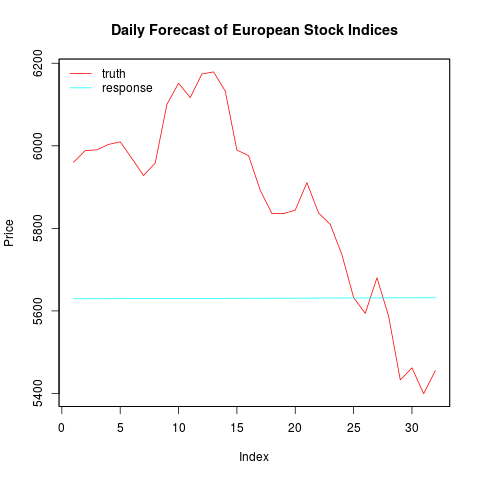
\includegraphics[width=\linewidth]{paper_figures/multfore_tune.png}
\centering
\caption{The forecast of the DAX Stock Index against the true values}
\label{fig:multfore_tune}
\end{figure}

This model only predicts a mean value for all forecasts, which may be due to poor performance of the stacked learner on top of the forecasts. The super learner trains on the forecasts of all the windowed cross-validations, though it does not understand that the forecast in period one is going to be better than the forecast at period $n$. Future research will create methods to correct this bias while training the super learner such as regressive weights over the forecast period, giving more weight to the most recent forecast.

\section{Conclusion}

The results of this paper show that creating a unified interface for forecasting models in \proglang{R} allows for better models through an automated methodology of resampling, preprocessing, model selection, stacking tuning, and training. Building on the broad range of forecasting packages available in \proglang{R}, automating tasks such as windowing cross-validation and model selection allow applied forecasters to spend less time dealing with the bureaucracy of modeling and more time testing new models. New methods such as multivariate stacked learners, Lambert W transforms, and the ability to create arbitrary AR($p,d$) machine learning models allows researchers to experiment with new ideas easily. While the example models here are not perfect, this was mostly due to time. It will be easy for researchers to beat the models created in this paper.

Future research based on this package would involve tuning these models to see how useful they are in the real world. The classification forecast learners made available in the forecasting extension of \pkg{mlr} is a growing field, and with the ease of making models in \pkg{mlr}, new research in this area can progress while being easily replicable. Updates to this package will include more multivariate and univariate forecast learners as well as new methods to stack models such as Bayesian averaging~\cite{bayesianAverage}.

%\small
\bibliography{thesisbib}{}
\bibliographystyle{plain}

\end{document}
